\chapter{构建材料模型}\label{ch:advanced}

\chapterlead{晶体中的缺陷、表面上的分子以及高分子混合物，都可以从少量清楚的结构信息逐步建立。本章介绍如何选择这些信息，如何读懂构建参数，以及怎样检查生成的模型。每个例子都把“形成一个合适的初始结构”作为目标，为后续计算留下清楚的起点。}

\section{从空间群建立晶体}
\index{Kongjianqun@空间群}

\subsection{理解非对称位点}

同一个晶体中的许多原子位置由对称操作联系。按空间群建模时，不必逐一输入全部原子；只需给出晶格、空间群和一组非对称位点，工具便会展开相应的等价位置。输入的是非对称位点，输出的是用于后续操作的完整晶胞，这一点是理解晶体构建器的关键。

空间群可以使用符号或编号表示。\ui{晶格矩阵}是一个可编辑的 $3\times3$ 表格：a、b、c 三行分别表示三个晶格矢量，x、y、z 三列表示矢量的笛卡尔分量，长度单位为 \AA。点击需要修改的单元格，逐格填写数值。每个非对称位点还需要元素、分数坐标和占据率。占据率 1 表示该元素完整占据位点；部分占据描述平均结构，在需要显式原子排列的计算中，通常还要进一步建立有序近似或合金模型。

\subsection{示例：面心立方铜}

本例以 $a=3.61\,\text{\AA}$ 建立常规面心立方 Cu 晶胞。这个晶格常数作为示例输入，读者可以用自己的实验或计算数据替换。

\begin{steps}
  \item 从\ui{项目浏览器}打开并激活晶体文档，选择顶部\ui{晶体建模}；在\ui{晶体与晶胞}区域打开\ui{对称性工具}，选择\ui{按空间群构建}。
  \item 在\ui{空间群符号或编号}中输入 \file{Fm-3m}。在\ui{晶格矩阵}表格中，将 a 行 x 列、b 行 y 列、c 行 z 列这三个对角单元格分别设为 3.61，其余六格均设为 0。
  \item \ui{元素符号}输入 Cu；\ui{非对称位置分数坐标}是一个文本框，输入 \literalinput{0 0 0}。\ui{非对称位置占位率}设为 1，\ui{展开位置重合容差}可先保持 $0.1\,\text{\AA}$。
  \item 预览并检查展开结果。常规面心立方晶胞应包含 4 个 Cu 位点，而不是只保留输入的那个位置。
  \item 单击\ui{应用}，在随后出现的结果窗口中阅读非对称位点与等价位点信息，核对元素、占据率和位置，再保存为\file{Cu-fcc}。
\end{steps}

本例只需要一个非对称位点，其余位置由空间群生成。出现展开后位点碰撞时，应先检查是否把同一组等价位置重复输入，而不是立即把碰撞容差调小。一个位置已由空间群展开后，再把它的等价位置作为独立输入，可能重复表达同一原子。

随书\file{Cu-fcc.cif}是按上述参数生成的四位点晶胞；\file{Cu-vacancy.cif}是后续空位枚举的一项结果，含三个位点。配套脚本可用于重新生成这两份结构。

\subsection{选择晶胞表示}

原胞用较少的原子表示晶体的平移周期；惯用胞则常使对称性和晶轴关系更直观。同一物质的两种晶胞可以包含不同原子数和不同形状，这并不表示成分发生变化。转换前后，宜同时检查化学式、体积与位点数，而不要仅比较屏幕上晶胞的大小。

\ui{分析对称性}、\ui{原胞}和\ui{惯用胞}使用位置与角度容差。默认位置容差为 $0.01\,\text{\AA}$，角容差为 $5^\circ$。这些参数用于判断轻微偏离的位置是否仍视为对称等价。对于已经发生真实畸变的结构，较大的容差可能把畸变解释为数值偏差，因此应结合模型来源理解识别结果。

\ui{转为 P1}将当前原子明确作为不受额外空间群关系约束的模型保存，适合随后进行局部编辑。转换保留原子位置及其几何对称性，后续编辑不再依赖原先声明的空间群关系。

\section{调整晶胞}

\subsection{选择正确的晶胞操作}
\index{Yingbian@应变}

\ui{编辑晶格}可以选择是否保持原子的笛卡尔位置；\ui{重定义晶胞}保持原子的笛卡尔位置，改变用于包围这些原子的晶格。这两个窗口都用 a、b、c 为行、x、y、z 为列的表格逐格编辑晶格。\ui{结构应变}则描述对整个结构的均匀形变。为了避免把不同的物理操作混在一起，先明确目标：是改变边界描述，还是使晶体中的全部距离随晶格一起缩放。

例如，在\ui{应变}文本框中输入 \file{0.01}，对三个方向都施加 0.01 的工程应变，表示长度乘以 1.01，而不是增加 $0.01\,\text{\AA}$。若只希望沿第一个方向拉伸，在同一个文本框中输入 \literalinput{0.01 0 0}。预览后检查晶格长度、角度与局部距离，再保存模型。

\ui{晶胞正交化}搜索满足长度、角度和原子数限制的整数超胞。它适合为需要近似正交盒子的后续流程准备模型，但不是任意晶格都能在有限搜索范围内精确变成正交胞。没有找到结果时，可适当扩大最大长度或原子数，或根据用途放宽角度容差；同时注意更大的超胞会增加后续计算量。

\section{筛选缺陷构型}
\index{Quexian meiju@缺陷枚举}

如果多个位点由晶体对称性联系，在它们上面创建同一种缺陷，可能得到等价模型。\ui{枚举点缺陷}把这类重复候选合并，并报告简并度。简并度表示有多少位置归入同一类，不表示该缺陷的能量高低。

\begin{steps}
  \item 打开前面的 \file{Cu-fcc} 模型，选择\ui{枚举点缺陷}。
  \item 缺陷类型设为 \file{vacancy}，以当前 Cu 晶胞中的位点作为候选范围。位置和角度容差先保持默认值。
  \item 单击\ui{应用}，在结果窗口查看候选表。理想常规面心立方 Cu 的4个位点相互等价，因此应归入一个空位候选，简并度为4。
  \item 检查候选的剩余原子数、组成与接触信息，再到项目浏览器的结构分组打开新增缺陷模型。保存当前项目，把原始铜晶体与缺陷结果一起保留。
\end{steps}

替位缺陷需要指定替换后的元素；间隙缺陷需要给出新增原子的坐标和坐标类型；反位缺陷涉及不同位点的元素交换。名称相近的操作，表达的是不同的结构变化。建立后先检查元素计数，再检查位置，通常比先看图像更容易发现输入错误。

\ui{生成 SQS 模型}用于把部分占据或混合组分表示为有限晶胞中的显式排列。工具以原子对关联函数为目标进行枚举或限时搜索，可设置超胞缩放和搜索时间。搜索预算影响候选质量与耗时；一次搜索产生的模型应连同组成、胞大小和搜索设置一起保留，以便比较。

\section{示例：建立 \headinglatin{Pt}(111) 表面}
\index{Biaomian moxing@表面模型}

\subsection{理解表面模型}

表面模型通常由有限厚度的晶体薄片与真空层组成，常称为 slab。面内方向周期重复，法向上用真空隔开相邻薄片。Miller 指数 $(hkl)$ 指定切割晶面；表面厚度、终止面和真空厚度共同决定最终模型。

\subsubsection{从米勒指数找到法向}

晶面法向由倒格矢确定。采用第\ref{ch:theory}章的倒格约定，表面对应的方向为
\begin{equation}
  \mathbf G_{hkl}=h\mathbf b_1+k\mathbf b_2+l\mathbf b_3,
  \qquad
  \hat{\mathbf n}=\frac{\mathbf G_{hkl}}{\|\mathbf G_{hkl}\|}.
  \label{eq:surface-miller-normal}
\end{equation}
式中，$\mathbf b_1,\mathbf b_2,\mathbf b_3$为倒格矢，单位为$\text{\AA}^{-1}$；$h,k,l$是无量纲整数，$\hat{\mathbf n}$是单位法向量。立方晶胞的三条边等长且正交，$(111)$法向与$\mathbf a+\mathbf b+\mathbf c$平行；本例的晶格轴沿全局坐标轴排列，因此也与全局$(1,1,1)$平行。斜晶胞一般没有这种对应关系，不能把米勒指数直接当作笛卡尔方向输入吸附物的定向参数。

构建后的表面晶胞以$\mathbf a,\mathbf b$为面内矢量，可用
\begin{equation}
  \hat{\mathbf n}_{\mathrm{slab}}=
  \frac{\mathbf a\times\mathbf b}{\|\mathbf a\times\mathbf b\|},
  \qquad H=|\mathbf c\cdot\hat{\mathbf n}_{\mathrm{slab}}|
  \label{eq:surface-normal-height}
\end{equation}
检查实际法向与晶胞高度。$H$是相邻周期表面之间沿法向的重复长度，并不总等于$\|\mathbf c\|$。把同一薄片的原子放在连续的周期映像中后，将原子位置投影到该法向，便可读出最外两层之间的跨度。它与构建窗口的最小厚度、完整重复单元厚度也应分别记录。

\begin{table}[H]
\centering
\caption{表面构建中几种长度的含义。}
\begin{tabularx}{\linewidth}{lX}
\toprule
量 & 怎样理解与核对\\
\midrule
最小薄片厚度 & 构建时用于选择完整重复单元的条件；不是直接指定层数。\\
原子层跨度 & 最外两层的法向距离；检查时先选取同一连续薄片。\\
法向胞高$H$ & 由式\eqref{eq:surface-normal-height}得到，包含薄片和周期间隔。\\
新增真空$\Delta$ & \ui{添加真空层}中沿第三晶格矢量增加的长度，不是最终总真空。\\
\bottomrule
\end{tabularx}
\end{table}

对于非正交输入，还要检查实际输出的法向、层数和周期间隔。斜晶胞的厚度换算与候选约简可能受到取向处理的影响，不宜只依据输入的最小厚度判断结果。本章的Pt例子从立方晶胞开始，并检查生成的表面。


最小薄片厚度并不等于严格的原子层数。为了保持晶格堆垛，工具需要选取完整的结构重复；不同晶面和终止面可能得到不同原子数量。输入 $8\,\text{\AA}$ 后，实际层数以生成模型为准。

本例先用\ui{按空间群构建}建立 Pt 晶体。空间群输入 \file{Fm-3m}；在\ui{晶格矩阵}表格中，逐格将 a 行 x 列、b 行 y 列和 c 行 z 列设为 3.92，其余六格设为 0。这样得到边长 $3.92\,\text{\AA}$ 的立方晶格。\ui{元素符号}输入 Pt，\ui{非对称位置分数坐标}文本框输入 \literalinput{0 0 0}，\ui{非对称位置占位率}设为 1。预览并检查体相晶胞，再从这一结构生成 (111) 表面。

\begin{table}[htbp]
\centering
\caption{Pt(111) 表面练习参数。}
\begin{tabularx}{\linewidth}{lX}
\toprule
参数 & 设置与含义 \\
\midrule
米勒指数（h k l） & 三个数值框从左到右分别填 1、1、1，选择 (111) 面。\\
最小表面厚度 & $8\,\text{\AA}$；最终检查实际层数与几何厚度。\\
最小真空厚度 & $10\,\text{\AA}$；用于本例构建演示。\\
表面模型居中 & 勾选，使薄片位于晶胞法向的中部。\\
使用最简表面晶胞 & 勾选，使用相应的简化表面重复单元。\\
终止候选序号 & 1；有多个候选时逐个比较。\\
\bottomrule
\end{tabularx}
\end{table}

\begin{steps}
  \item 激活 Pt 体相结构，在顶部\ui{晶体建模}的\ui{表面与界面}区域打开\ui{表面建模}，选择\ui{构建表面模型}。
  \item 按表输入参数，预览表面。先沿接近表面法向观察面内排列，再转到侧面观察厚度和真空。
  \item 在参数窗口中将终止候选序号设为1。应用后，在结果窗口查看终止候选信息，结合表面元素、堆垛和研究目的比较各项。
  \item 检查晶胞边框和原子是否相符，记录实际原子数与层数，保存为\file{Pt111-slab}。若要换用其他终止，回到原始体相，再打开命令并修改终止候选序号；候选表本身只用于查看。
\end{steps}

% 第8章Pt(111)构建参数步骤后插入；本片段不修改第8章。
% 实际Online截图，仅以LaTeX裁切，不依文件名推定浏览器缩放。
\begin{figure}[H]
\centering
% 原图3024×1758；(980,735,2045,1290)，1065×555；107mm约253ppi。
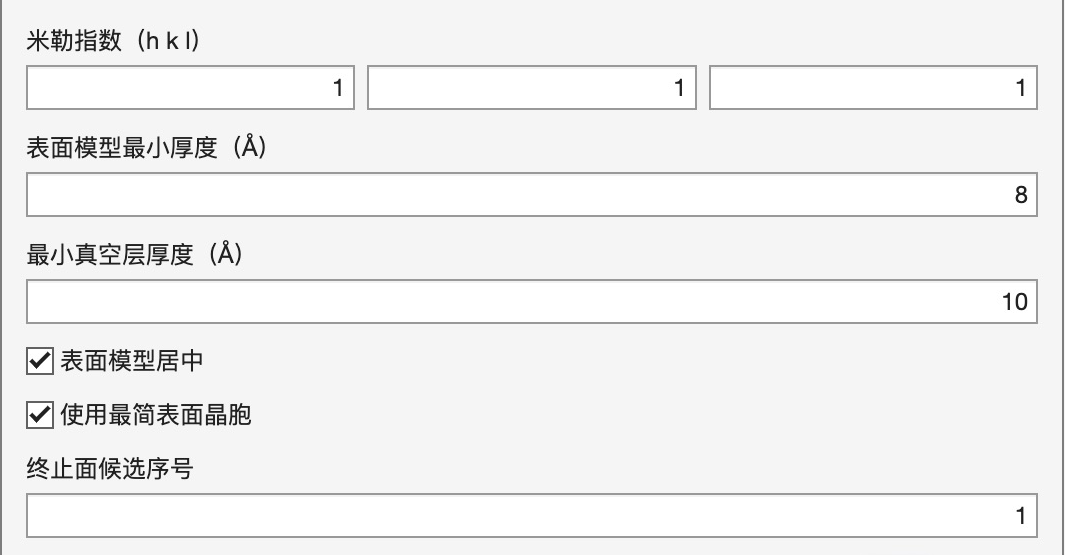
\includegraphics[width=107mm]{publication-assets/crop-e2fa9f70b6bcca245a04.png}
\par\vspace{2mm}
% 同图独立预览提示(975,1460,1520,1495)，545×35；54mm约256ppi，无右侧指针。

\includegraphics[width=54mm]{publication-assets/crop-f2ece60af591133fac37.png}
\caption{导入\file{Pt-fcc.cif}后构建Pt(111)表面的参数。米勒指数依次为1、1、1，最小表面厚度为$8\,\text{\AA}$，最小真空层厚度为$10\,\text{\AA}$；启用居中与最简表面晶胞，终止面候选序号为1。下方显示预览提示。}
\label{fig:pt111-slab-parameters}
\end{figure}


随书\file{Pt-fcc.cif}与\file{Pt111-slab.cif}分别提供这一体相和表面模型。本组参数得到 4 个独立位点、4 个几何层。沿表面法向，晶胞周期高度约为 $20.3689\,\text{\AA}$，最外两层原子平面的跨度约为 $6.7896\,\text{\AA}$，相邻周期薄片的最外原子平面之间相隔约 $13.5793\,\text{\AA}$。构建厚度按晶体重复单元选取，与最外原子坐标的差值不是同一种计量。测量时应沿表面法向投影；斜晶胞的第三条晶格矢量长度不能直接当作真空厚度。

\subsection{固定底层原子}
\index{Guding yuanzi@固定原子}
\index{Zhenkong@真空层}

表面弛豫中常保留底部若干层，以近似较深处的体相约束。表面构建后，工具可以识别几何层。打开\ui{固定原子}，将底部几何层数设为 1，可选择最底部一层。若使用当前选择而不是自动底层，应按界面设置将底层数置为 0，再明确选择需要固定的位点。

固定标记保存在模型中。提交计算时，在相应任务设置中启用所需约束。对于较厚薄片，也可以固定多层；初次练习时先固定一层并查看层的范围，便于理解。

\subsection{留出真空层}

\ui{添加真空层}沿第三条晶格矢量增加空间，输入的是新增厚度。若该矢量与表面法向倾斜，新增长度在法向的投影会小于输入值；本例使用法向晶胞练习。例如再输入 $5\,\text{\AA}$，表示在当前模型基础上继续增加空间，不是将总真空强制设为 $5\,\text{\AA}$。应用后从侧面检查晶胞与薄片的位置关系。吸附质或溶剂加入后，原先看起来充足的真空还可能被占去一部分，因此应再次查看完整模型。

新增真空的几何关系为
\begin{equation}
  \mathbf c'=
  \frac{\|\mathbf c\|+\Delta}{\|\mathbf c\|}\,\mathbf c,
  \qquad
  \Delta H=\Delta\,
  \left|\frac{\mathbf c}{\|\mathbf c\|}\cdot\hat{\mathbf n}_{\mathrm{slab}}\right|.
  \label{eq:vacuum-addition-projection}
\end{equation}
$\Delta$和$\Delta H$的单位都是\AA。前者是输入的新增长度，后者是法向胞高的增加量；点积给出的比例介于0和1之间。例如，第三晶格矢量沿全局$z$，表面法向沿$(1,1,1)$时，输入$2\,\text{\AA}$只会增加约$2/\sqrt{3}=1.155\,\text{\AA}$的法向胞高。图\ref{fig:surface-vacuum-geometry}中的$\Delta\mathbf c=\mathbf c'-\mathbf c$是长度为$\Delta$的增量，$\Delta H$是它的法向投影长度；将$\mathbf c$先整理到法向后，长度与实际间隔便容易对应。



\begin{steps}
  \item 重新导入\file{Pt111-normal-c.json}，保留一份未修改的薄片。这份输入的第三条晶格矢量已沿表面法向。在\ui{晶体建模}的\ui{表面建模}中打开\ui{添加真空层}。
  \item 新增厚度设为 $5\,\text{\AA}$。先预览，从侧面比较薄片与外框，确认改变的是薄片外的空间。
  \item 应用后再次核对 Pt 位点数和薄片内部几何；增加真空不应增加 Pt 原子，也不应拉大薄片内部的层间距。
  \item 另存为\file{Pt111-extra-vacuum}，与原始薄片分别保留。后面的吸附练习仍从指定的原始文件重新开始。
\end{steps}

\begin{figure}[H]
\centering
\begin{tikzpicture}[x=1mm,y=1mm,font=\sffamily\small,>=stealth]
  \foreach \shift in {0,65} {
    \fill[paleblue] (\shift+12,15) rectangle (\shift+44,25);
    \draw[teal] (\shift+12,15) -- (\shift+44,15);
    \draw[teal] (\shift+12,25) -- (\shift+44,25);
    \foreach \x in {16,25,34,43} {
      \fill[brand] (\shift+\x,18) circle (1.3);
      \fill[teal] (\shift+\x-2,22) circle (1.3);
    }
    \draw[->,brand,line width=.7pt] (\shift+12,6) -- (\shift+45,6)
      node[right] {$\mathbf a$};
    \draw[densely dashed,muted] (\shift+12,25) -- (\shift+12,53);
  }
  \node[text=brand] at (29,65) {倾斜的第三晶格矢量};
  \node[text=brand] at (94,65) {第三晶格矢量沿法向};
  \draw[->,brand,line width=.8pt] (12,6) -- (34,44)
    node[pos=.55,right] {$\mathbf c$};
  \draw[->,teal,line width=1pt] (34,44) -- (41,56)
    node[pos=.6,right] {$\Delta\mathbf c$};
  \draw[densely dashed,muted] (34,44) -- (51,44);
  \draw[densely dashed,muted] (41,56) -- (51,56);
  \draw[<->,teal] (49,44) -- (49,56);
  \node[anchor=south,text=teal,font=\sffamily\footnotesize] at (48,57) {$\Delta H$};
  \draw[->,muted,line width=.7pt] (6,28) -- (6,49)
    node[above] {$\hat{\mathbf n}$};
  \draw[->,brand,line width=.8pt] (77,6) -- (77,44)
    node[pos=.52,left] {$\mathbf c$};
  \draw[->,teal,line width=1pt] (77,44) -- (77,56)
    node[right] {$\Delta H=\Delta$};
  \node[align=center,font=\sffamily\footnotesize] at (29,-4)
    {法向增加量小于沿 $\mathbf c$ 的新增长度};
  \node[align=center,font=\sffamily\footnotesize] at (94,-4)
    {输入的新增长度就是法向增加量};
\end{tikzpicture}
\caption{添加真空层时的方向关系（截面示意）。薄片内部的相对位置保持不变，第三晶格矢量沿原方向伸长，工具同时将薄片重新居中；只有当它垂直于表面时，新增长度才全部用于增大法向间隔。}
\label{fig:surface-vacuum-geometry}
\end{figure}


\section{在表面放置吸附物}
\index{Xifu@吸附建模}

\subsection{确定吸附位置}

表面吸附建模需要回答三个问题：放在哪里、以哪个原子连接、朝向哪边。顶位（ontop）位于表面原子上方，桥位（bridge）位于两个表面原子之间，空位（hollow）位于若干表面原子围成的区域中。分子内部的锚定原子决定哪一个原子放在给定高度；取向原子则帮助确定分子的方向。

先用\ui{寻找吸附位点}观察候选位置，可以把抽象的位点名称与当前表面对应起来。默认高度为 $2\,\text{\AA}$。位点是生成初始构型的几何参考，并不表示分子在该处已经达到稳定吸附。

\subsection{为吸附练习整理晶胞}

先重新导入未经修改的\file{Pt111-slab.cif}。本节不使用前一节额外增加真空后的结构。这个表面的法向沿全局坐标的 $(1,1,1)$，原晶胞的 $c$ 矢量却沿全局 $z$ 方向。当前参数命令沿 $c$ 方向增加锚点高度，因此先把 $c$ 调整到表面法向，可以使输入高度与侧视图中的垂直距离一致。

打开\ui{重定义晶胞}，保留 $a$、$b$ 两行，只将 $c$ 行的 $x$、$y$、$z$ 三项分别设为 11.76、11.76、11.76，单位为 \AA；保持原子的笛卡尔位置。这里采用的是 $c_{\mathrm{new}}=c+6a+6b$，没有扩胞，仍有 4 个 Pt 位点。新的 $c$ 垂直于表面，面内 $a$ 与 $b$ 之间仍为 $60^\circ$。也可以直接导入随书的\file{Pt111-normal-c.json}，从已经整理好的晶胞开始。

从侧面查看薄片，再显示晶胞边框：$c$ 应沿表面向外，薄片内部的层间位置保持不变。对于其他表面，应根据其面内矢量确认法向，不要直接套用本例的三项坐标。

\subsection{示例：交互放置 \headinglatin{O--H} 片段}

交互方式适合观察分子如何接近表面。它允许一边拖动完整片段，一边检查高度、取向和接触。

\begin{steps}
  \item 打开已整理晶胞的 \file{Pt111-normal-c}，按 O 进入吸附物放置，选择 O--H 片段。片段栏也可使用项目中的分子或用户片段。
  \item 从表面原子向外拖动，建立表面位点与片段锚点之间的关系。调整视图，使拖动方向容易判断。
  \item 左键拖动改变整个片段的朝向；Alt+左键拖动调整锚定距离；右键拖动使片段绕锚定方向旋转。
  \item 检查 O--H 内部连接是否保持，片段是否与邻近表面原子过近。预览合适后按 Enter 或\ui{应用}提交。
  \item 保存为独立吸附模型。若要调整放置方式，可撤销后重新操作。
\end{steps}

\subsection{示例：按参数向外放置 \headinglatin{O--H}}

参数方式便于记录和重复相同的构型。随书\file{oh-fragment.mol}含 O、H 两个原子和一条单键，O--H 长度为 $0.96\,\text{\AA}$。先把它导入项目，再重新导入未经吸附修改的\file{Pt111-normal-c.json}并激活新导入的宿主，从干净的四位点薄片开始。

\begin{steps}
  \item 打开\ui{放置吸附物}，在\ui{项目吸附物}下拉菜单中选择导入的 O--H 分子。
  \item 位点类型选择顶位（ontop），候选序号为 1，\ui{锚点高度（Å）}设为 2。
  \item 锚定原子设为 1，即 O；取向原子设为 2，即 H。在方向的三个数值框中分别填 1、1、1，使 O 指向 H 的方向与本例表面法向一致。最小允许距离保持 $0.5\,\text{\AA}$。
  \item 预览后从侧面检查：O 应位于选定 Pt 原子的外侧，H 在更远的一端，再单击\ui{应用}。
  \item 本例输入含负的分数坐标。为使宿主与吸附物在同一晶胞内查看，打开\ui{构建超胞}，三个缩放值都填1并应用。这一步把等价位点归入单位晶胞，不扩大模型；晶格和6个独立位点保持不变。
  \item 将结果改名为\file{Pt111-OH-outward}并保存。打开晶胞边框，从侧面检查O--H朝向；边界映像可能使同一片段显示多次，应以摘要中的6个独立位点核对组分。
\end{steps}

% Online实际参数放置与归胞后的侧视；只裁切原JPEG，不修改像素。
\begin{figure}[H]
\centering
% 3024×1758；(980,620,2045,1480)，1065×860；107mm约253ppi。
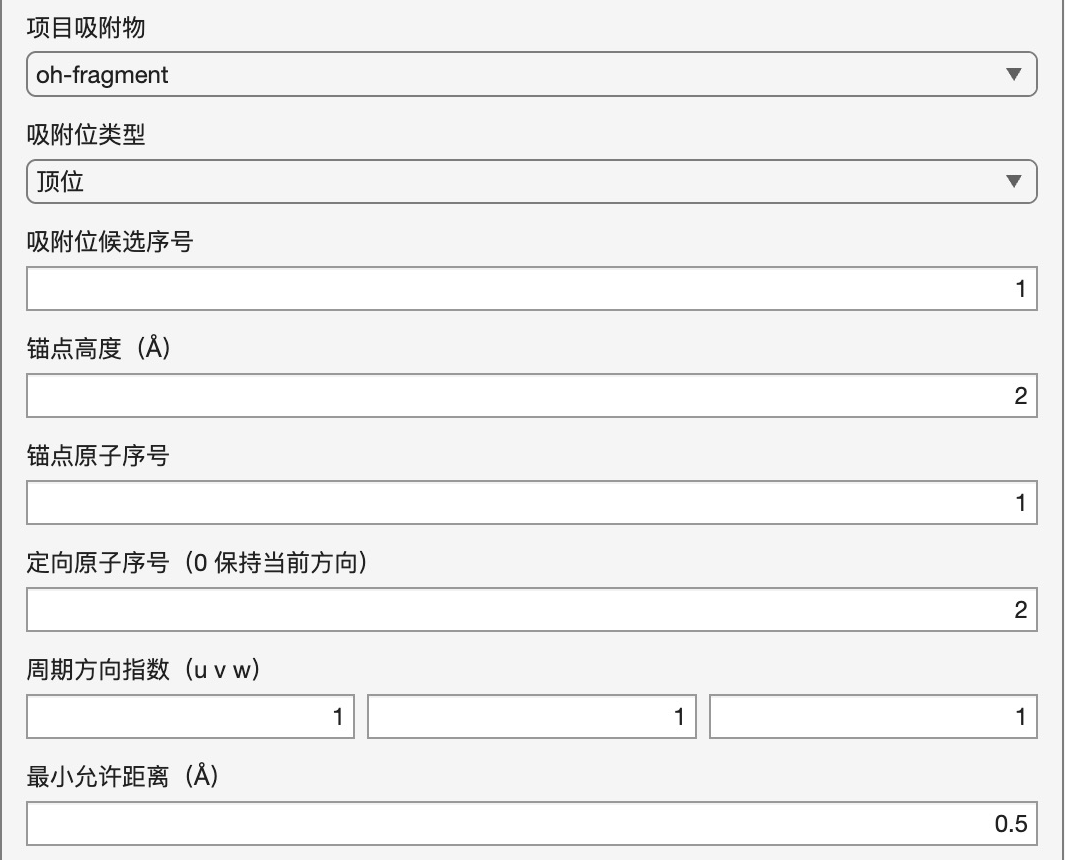
\includegraphics[width=107mm]{publication-assets/crop-c02e14aa8762e8947bbe.png}
\caption{向外放置O--H的参数。选择项目中的\file{oh-fragment}，顶位候选1，锚点高度$2\,\text{\AA}$，锚定原子1、定向原子2，周期方向指数依次为1、1、1，最小允许距离$0.5\,\text{\AA}$。本例先将宿主的$c$调整为表面法向。}
\label{fig:pt111-oh-parameters}
\end{figure}

\begin{figure}[H]
\centering
\begin{minipage}[t]{80mm}
\vspace{0pt}
% 完整晶胞(1000,360,2020,1685)，1020×1325；80mm约324ppi。
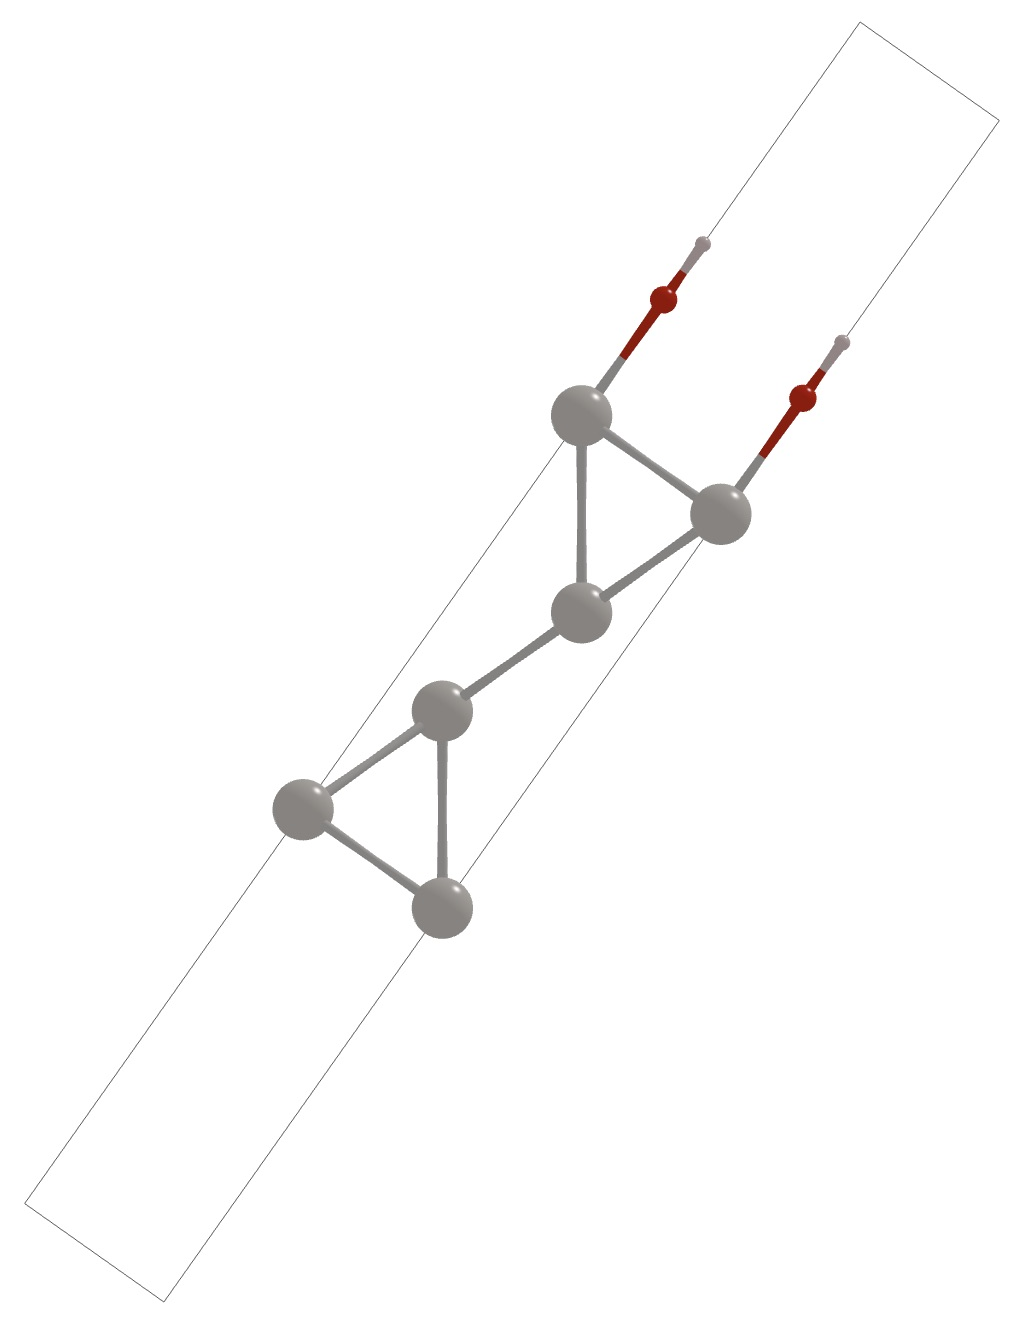
\includegraphics[width=\linewidth]{publication-assets/crop-c201c0495d5d847c2fd3.png}
\end{minipage}\hfill
\begin{minipage}[t]{40mm}
\vspace{0pt}
% 独立摘要(40,330,445,560)，405×230；40mm约257ppi。
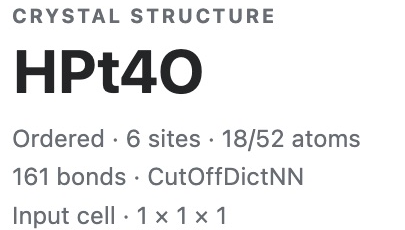
\includegraphics[width=\linewidth]{publication-assets/crop-5caa5064e4762ffc4974.png}
\end{minipage}
\caption{应用吸附放置并以$1\times1\times1$单位超胞归胞后的结构侧视。模型组成为$\mathrm{Pt_4OH}$，含6个独立位点；画面中的两个O--H为同一片段的周期映像。图中展示吸附物放置后的初始结构。}
\label{fig:pt111-oh-side}
\end{figure}


参考结果含 $\mathrm{Pt_4OH}$，共 6 个位点。O 距顶层平面 $2.00\,\text{\AA}$，H 距顶层平面 $2.96\,\text{\AA}$，O--H 长度保持 $0.96\,\text{\AA}$。随书\file{Pt111-OH-outward.cif}可用来比较晶胞和原子位置；片段的显式单键保存在输入 MOL 文件中。若将取向原子改为 0，工具会保留片段原有朝向，因此相同锚点高度不一定得到同一取向。

随书\file{Pt111-OH-Online-050.json}保存归胞后的六个位点，其周期几何与上述结构相同，可直接用于查看和继续建模。吸附能需通过后续计算求得。

\subsection{批量比较吸附构型}

\ui{吸附构型定位器}可以枚举位点、高度和转角，并按评分保留一组候选。先重新导入未经吸附修改的\file{Pt111-normal-c.json}，激活新导入的四位点宿主，再选择上述 O--H 分子。在\ui{位点类型}文本框中输入 \literalinput{ontop bridge hollow}，在\ui{候选高度（Å）}文本框中输入 \literalinput{1.8 2.1 2.4}，表示比较 $1.8$、$2.1$、$2.4\,\text{\AA}$ 三个高度。锚定原子设为 1，取向原子设为 0；旋转步长设为 $30^\circ$，最小接触距离 $0.6\,\text{\AA}$，最多保留 200 个候选，种子为 0。评分模型使用默认几何接触评分。

本组参数对应 144 个候选，各构型保持 O--H 长度，锚点位于指定的法向高度。\file{Pt111-OH-candidate-1.json}保存几何评分第一项：hollow 类型的候选 2，高度 $2.4\,\text{\AA}$，转角 $60^\circ$。可以先将它与前面的顶位模型比较，再观察其他候选的锚点和转角。

这些值用于理解搜索范围。分子较大时，可先减少高度与转角组合，确认锚点设置正确，再扩大搜索。候选表中选定一项后，先\ui{预览}，比较不同构型，再\ui{应用}所需候选。对后续需要分别弛豫的构型，应保留为多个清楚命名的模型。

默认几何接触评分反映构型的几何适合程度；可选的 UFF 范德华相互作用能是在刚性模型下的相互作用估计。两者适合筛选初始结构，不能替代弛豫后的吸附能。记录研究结果时，同时说明构型来源与后续计算方法。

\section{处理表面边界}

\subsection{钝化未饱和表面}

\ui{表面钝化}根据未饱和配位添加原子。参数包括钝化元素、键长、处理上表面或下表面，以及表面探测深度。默认元素为 H、键长 $1.1\,\text{\AA}$、同时处理两侧、探测深度 $1.5\,\text{\AA}$。对于不同材料，应按目标化学结构选择键长和配位数。目标配位设为 0 时由工具推断；已知表面化学时可以明确指定。

\subsection{建立溶剂层}

\ui{添加溶剂层}把项目中的溶剂分子装填到表面上方。应先准备并检查单个溶剂分子，再设置分子数、层厚、表面间隔和剩余真空。例如，20 个分子、层厚 $10\,\text{\AA}$、表面间隔 $2\,\text{\AA}$、剩余真空 $5\,\text{\AA}$，构成一组容易查看的练习输入。接触容差和随机种子影响装填结果；完成后从侧面检查分子层范围，再从上方检查局部堆积。

\section{构建异质结}\label{sec:heterojunction}
\index{Cengpipei@层匹配}
\index{Yizhijie@异质结}

\subsection{理解两种材料的共同晶胞}

异质结由两种不同材料相接形成。对层状界面，可以把两侧材料分别准备为薄片，再沿法向叠放。两种材料原来的晶格通常不同；要把它们放入同一个周期计算模型，需要找到共同的面内晶胞，并决定允许多少形变。这个共同晶胞既描述界面的重复方式，也决定一次计算包含多少原子。

本节的\ui{堆叠异质结构}用于这类上下叠放的界面。它比较面内超胞与旋转，随后按指定间距组装两部分。石墨烯/h-BN 是便于观察的小例子；从块体材料建立薄膜界面时，先分别用\ui{构建表面模型}准备需要相接的晶面，检查每一侧的层数、终止面和组成，再进行匹配。材料名称相同并不意味着表面取向已经相同，晶面选择应先于界面组装。

面内应变表示原有晶格为了共用一个周期而改变了多少，层间距表示两部分初始分开的距离，面内平移则改变局部原子如何上下对齐。三个量各有作用。建立几何模型后，还可以在同一组计算条件下比较不同间距和堆垛；界面电荷转移、能带对齐等性质由后续电子结构计算分析。

\subsection{按位移插入结构}

\ui{插入结构}把项目中的另一结构放入当前模型，可指定笛卡尔平移向量和最小原子间距。它适合已经知道两部分相对位置的情况。插入后应检查晶胞、组成和跨边界的邻近接触。

\subsection{寻找面内晶格匹配}

\ui{堆叠异质结构}进一步搜索面内晶格匹配。需要选择顶层结构，给定层间距、总真空、最大面内应变、重复范围和旋转范围。默认层间距 $3.35\,\text{\AA}$ 只是界面初值，不能通用于所有材料。最大应变 0.03 表示 3\%，是无量纲约束；候选可以按应变、面积或原子数排序。

比较候选时，可以先看应变是否合理，再看晶胞面积与原子数能否满足计算规模。最小应变候选不一定也是最小模型。选定候选后检查两层的面内方向、层间距离和真空，再为不同堆垛分别保存结构。

\subsection{练习：比较直接插入与层匹配}

随书\file{graphene-layer.json}是一个含两个 C 位点的石墨烯层，面内晶格常数为 $2.46\,\text{\AA}$，盒高为 $15\,\text{\AA}$。面内周期重复，法向为非周期。先将它导入两次并分别命名为\file{bottom}和\file{top}，即可用同材双层练习几何操作。

直接插入时，激活底层，打开\ui{插入结构}，将项目中的另一结构设为顶层。在\ui{插入位移（笛卡尔，Å）}的三个数值框中，从左到右分别填 0、0、3.35，最小距离保持 $0.5\,\text{\AA}$。结果应有 4 个位点，两层相隔 $3.35\,\text{\AA}$，原盒高仍为 $15\,\text{\AA}$。随书\file{graphene-inserted.json}保留了这个状态。

另从原始底层开始，打开\ui{堆叠异质结构}，仍以\file{top}作为另一结构。层间距设为 $3.35\,\text{\AA}$，总真空为 $15\,\text{\AA}$，最大面内应变为 0.03，最大面内重复数为 2，最大旋转搜索角为 $0^\circ$，候选按面积排序。

在参数窗口将\ui{界面候选序号}设为1，预览并应用，再查看结果候选表。随书参考结果列出10个候选，候选1的应变为0、预计4个位点。应用后得到盒高 $18.35\,\text{\AA}$、层间距 $3.35\,\text{\AA}$ 的双层，对应\file{graphene-stacked.json}。比较两种结果，可以看到直接插入保留原盒子，而层匹配构建按薄片与总真空重新安排法向尺寸。

候选列表还可能包含高于指定应变上限的组合；列出不表示可以直接应用。本例候选 2、3 的应变约为 52.49\%，应排除；候选 4、5、6 接近零应变，但需要 8 个位点。先检查约束，再选择面积或规模合适的候选，比只看排列图像更可靠。

\subsection{示例：石墨烯与 h-\headinglatin{BN} 的层匹配}

两种材料的面内尺寸通常略有差别。本例将石墨烯与六方氮化硼（h-BN）叠放，观察匹配时的应变。\file{hBN-layer.json}是含 B、N 各一个位点的理想单层，面内晶格常数为 $2.50\,\text{\AA}$；石墨烯的相应数值为 $2.46\,\text{\AA}$。两份输入的法向盒高均为 $15\,\text{\AA}$。

\begin{steps}
  \item 将\file{graphene-layer.json}与\file{hBN-layer.json}导入同一项目。激活新导入的\file{graphene-layer}，打开\ui{堆叠异质结构}，在\ui{上层结构}下拉菜单中选择\file{hBN-layer}。
  \item 层间距设为 $3.35\,\text{\AA}$，总真空设为 $15\,\text{\AA}$，最大面内应变设为 0.03。
  \item 最大面内重复数设为 1，最大旋转搜索角设为 $0^\circ$，候选按应变排序。先限制到这个小范围，便于看清两种晶格如何匹配。
  \item 在参数窗口将\ui{界面候选序号}设为1，预览并应用，再从侧面检查层间距。应用后出现的候选表只有一项：面内应变为0.016，即1.6\%，预计4个位点。
\end{steps}

候选表用于查看各组匹配，并不在表内提供切换构型的应用按钮。比较其他候选时，先撤销到原始底层，或重新导入底层，再打开同一命令并填写需要的候选序号。不要在已经组装的双层上继续叠加。

结果\file{graphene-hBN-stacked.json}含 $\mathrm{C_2BN}$，h-BN 的面内晶格匹配到石墨烯晶格；层间距为 $3.35\,\text{\AA}$，法向盒高为 $18.35\,\text{\AA}$。与同材双层相比，本例需要有限的面内形变才能共用一个周期晶胞。后续可以扩大重复与旋转范围，比较更大的匹配晶胞，并分别保存准备计算的构型。这里的层间距是建模初值，弛豫后的距离需由相应计算确定。

\section{构建扭转双层}\label{sec:twisted-structures}
\index{Niuzhuan shuangceng@扭转双层}
\index{Moer chaojingge@莫尔超晶格}

\subsection{从相对转角到共同周期}

将两张石墨烯单层重叠，再使其中一层绕法向转动，局部的原子对齐关系就会随位置改变：有些区域接近原子上下相对，有些区域接近一层原子落在另一层六元环中心。把视野扩大，可以看到这些局部排列组成较大的重复图案，称为莫尔图案。

用于周期计算的模型还需要一个共同晶胞。上层不能只在原来的小晶胞中任意旋转，否则越过晶胞边界后，两层的排列通常接不上。\ui{扭转莫尔超晶格}为两层分别选择整数超胞，使它们能够放入同一面内周期。输入的目标角用于寻找合适的匹配，最终模型则由一组具体的整数关系确定。

本节使用约 $21.7868^\circ$ 的石墨烯双层作为第一例。这个转角对应较小的共同周期，结果只有 28 个碳位点，便于同时观察两层和晶胞。先完成这个例子，再尝试较小转角，能够更清楚地理解角度、周期和模型规模之间的关系。

\subsection{准备上下两层}

本工具使用六方面内原胞：两个面内晶格矢量等长，夹角为 $60^\circ$ 或 $120^\circ$。本例的单层石墨烯包含两个 C 位点，面内晶格常数为 $2.46\,\text{\AA}$，盒高为 $15\,\text{\AA}$。两个面内方向周期重复，法向为非周期。

随书的\file{twist-graphene-bottom.json}与\file{twist-graphene-top.json}来自同一份单层输入，分别供底层和上层使用。它们与前面\file{graphene-layer.json}的几何相同。两份文件分开命名，是为了让项目中的角色一目了然，不表示两层已具有不同转角。

\begin{steps}
  \item 把两份 JSON 导入同一项目，分别将结构命名为\file{twist-bottom}和\file{twist-top}。
  \item 打开底层的三维文档，检查它只有两个模型位点。屏幕上用于显示周期连接的映像原子可以多于两个。
  \item 查看晶格，确认面内长度均为 $2.46\,\text{\AA}$、夹角约为 $120^\circ$。再检查上层具有相同的晶格和组成。
  \item 激活\file{twist-bottom}。在顶部\ui{晶体建模}的\ui{表面与界面}区域打开\ui{界面建模}，选择\ui{扭转莫尔超晶格}。
  \item 在\ui{上层结构}下拉菜单中选择\file{twist-top}。这里选的是项目中已有的结构，不是在输入框中填写磁盘路径。
\end{steps}

第一次练习应从这两张原始单层开始。前面已经插入或堆叠过的双层可另行保留，不能再把它当成一张原始单层送入本例。

\subsection{填写一组小规模参数}

\begin{table}[htbp]
\centering
\caption{28位点石墨烯扭转双层的练习参数。}
\begin{tabularx}{\linewidth}{lX}
\toprule
参数 & 本例输入与含义\\
\midrule
上层结构 & 在下拉菜单中选择\file{twist-top}。\\
角度（度） & 输入\literalinput{21.786789}，作为目标相对转角。\\
层间距（Å） & 输入 3.35，规定两张单层之间的初始间隔。\\
总真空层厚度（Å） & 输入 15，规定薄片之外的总空白高度。\\
允许的最大面内应变 & 输入 0.03，即 3\%。\\
最大原子数 & 输入 200，限制生成模型的总位点规模。\\
最大周期匹配指数 & 输入 6，限定整数匹配的搜索范围。\\
\bottomrule
\end{tabularx}
\end{table}

\ui{角度（度）}是一个数值框，输入的是度数；不需要再写度符号。\ui{层间距}和\ui{总真空层厚度}也都是长度数值。最大应变则是比例，0.03 表示 3\%，不能把 3 直接填作同一个要求。

最大原子数不是要求软件一定生成 200 个原子，而是允许的上限。最大周期匹配指数也不是沿某个方向简单重复 6 次。工具会在这个范围内寻找整数匹配，综合考虑目标角偏差、应变和结构大小，再选出一组结果。因此，这两个上限与\ui{构建超胞}中的三个重复倍数有不同含义。

本命令内部选择一组匹配，不提供\ui{堆叠异质结构}那样的候选排序和候选序号字段。填写完参数后，应检查生成结构的实际规模和相对取向；需要比较其他匹配时，保留原始两层，分别生成和保存各组参数的结果。

\begin{steps}
  \item 按表填写参数，先使用\ui{预览}检查。模型应从两个位点的单层变成两层组成的较大周期结构。
  \item 沿接近表面法向观察，检查两层的六元环排列已经相对转动；转到侧面，确认仍然只有两层，层间没有意外插入其他原子。
  \item 检查模型位点总数应为 28。面内晶胞扩大后，查看器的显示映像数仍可能多于这个数。
  \item 应用后把结果命名为\file{graphene-twist-21p786789}，保存项目。保留两份输入单层，使后续比较可以从同一起点开始。
\end{steps}

\begin{figure}[H]
\centering
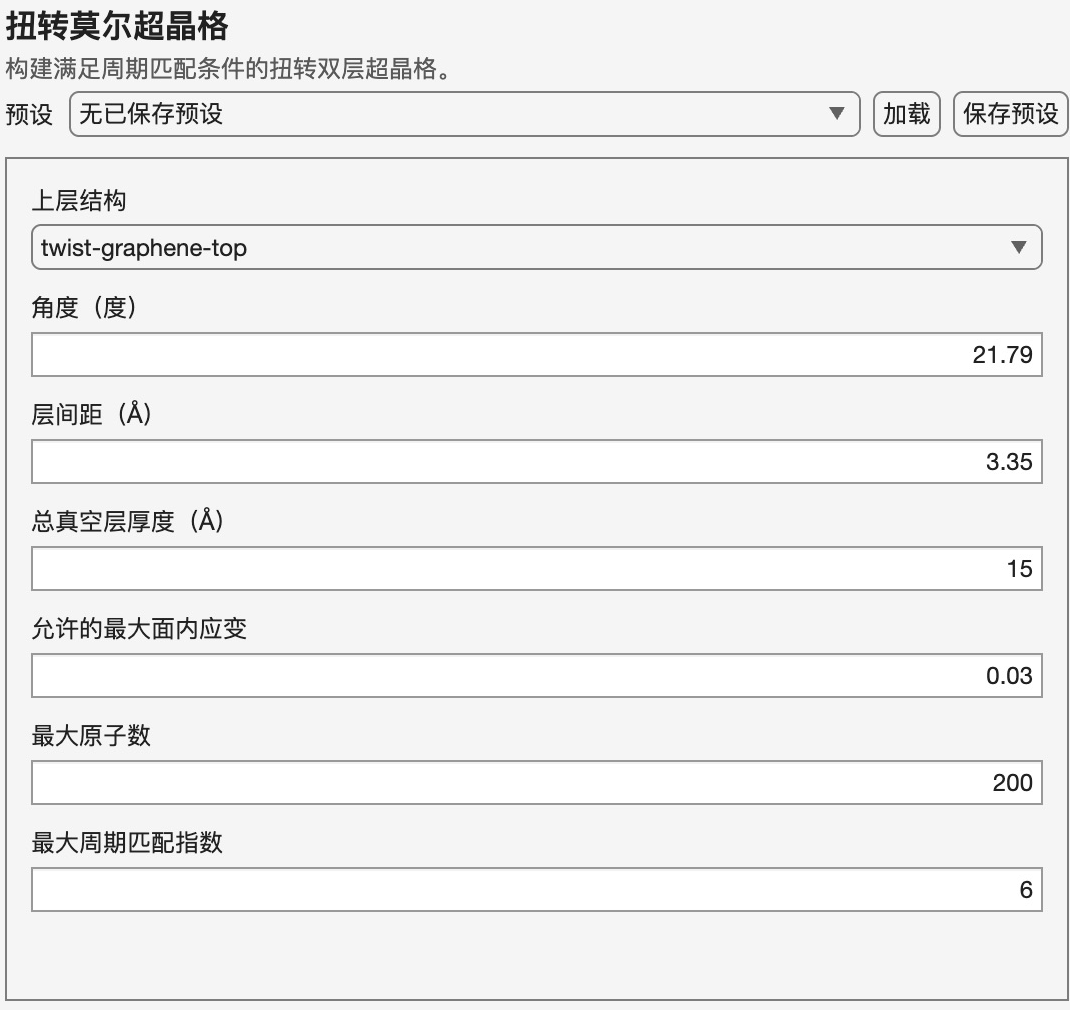
\includegraphics[width=107mm]{publication-assets/crop-7c221ceb9a35fdad53a3.png}
\par\vspace{2mm}

\includegraphics[width=60mm]{publication-assets/crop-faecdf5879e359505e34.png}
\caption{扭转参数与预览结果。目标角输入21.786789度；数值框失去焦点后按显示精度呈现为21.79。上层在图中保留导入时的名称\file{twist-graphene-top}，对应本节的\file{twist-top}；预览生成28个位点。}
\label{fig:online-twist-parameters}
\end{figure}

\begin{figure}[H]
\centering
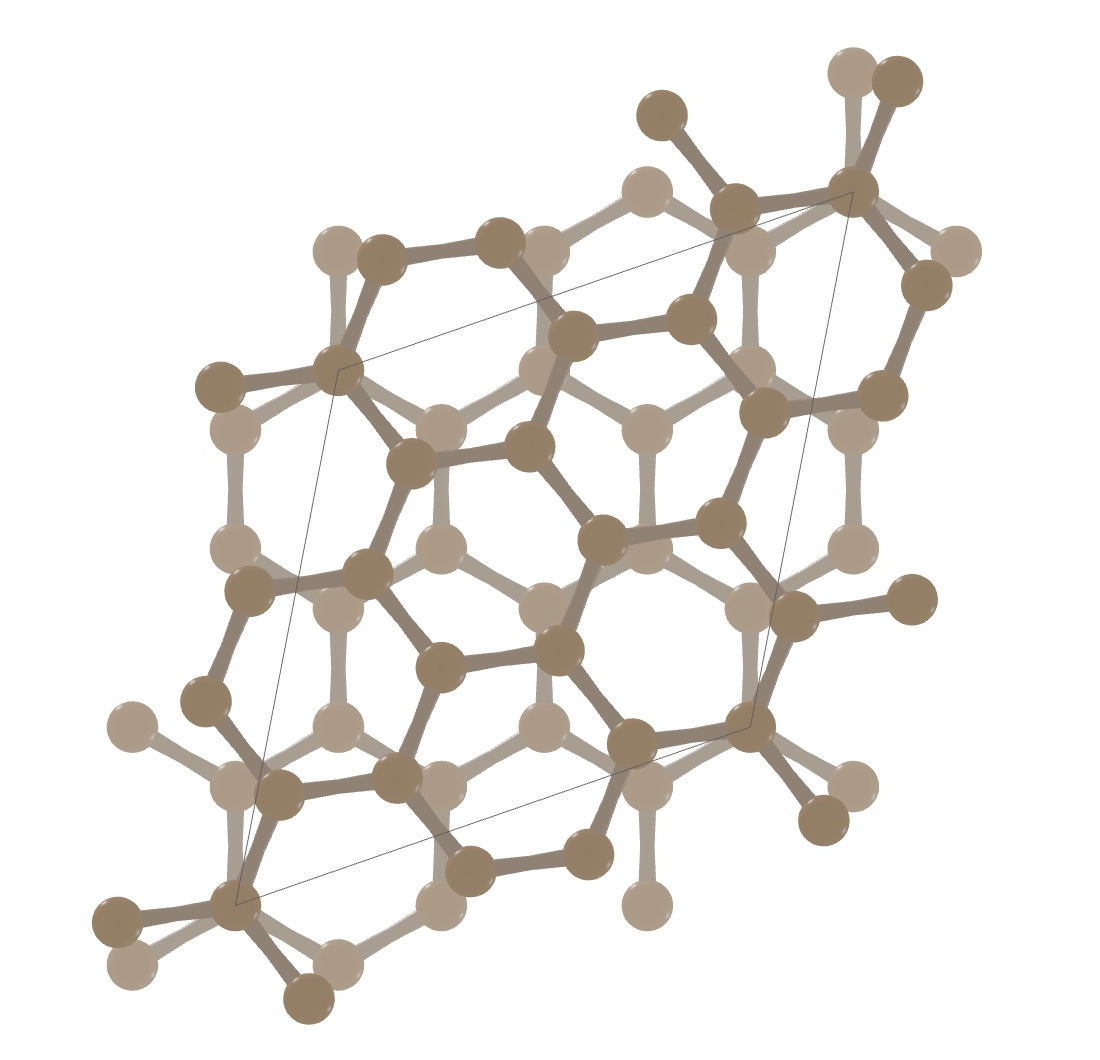
\includegraphics[width=93mm]{publication-assets/crop-89eb072a4598add87b05.png}
\caption{石墨烯扭转双层的法向视图。两层的六元环相对转动；28个模型位点按当前周期范围显示为68个原子。}
\label{fig:online-twist-top}
\end{figure}

\subsection{读懂生成的晶胞}

随书\file{graphene-twist-21p786789.json}是按上述参数得到的参考结构，另提供几何交换用的同名 CIF。模型有 28 个 C 位点，分为两层，每层 14 个。与原始每层两个位点相比，每一层的面内面积扩大为原来的 7 倍。

面内两个晶格矢量等长，均约为 $6.508548\,\text{\AA}$。相应面积约为 $36.6859\,\text{\AA}^2$。本例的新面内夹角为 $60^\circ$；输入原胞的夹角为 $120^\circ$，两者是不同的晶格基底表示，不能只凭角度改变就判断晶体被拉歪。核对长度、面积、位点数与两层的周期连接，应当放在一起进行。

对于这组石墨烯输入，周期边长也可用 $\sqrt{7}\times2.46\,\text{\AA}$ 核对，约为 $0.651\,\mathrm{nm}$。这里的周期描述共同晶胞在面内的重复长度，不是层间距离，也不是某条 C--C 键长。模型中每层最短近邻距离仍约为 $1.420282\,\text{\AA}$，与输入单层一致。

从侧面看，两层相隔 $3.35\,\text{\AA}$，法向胞高为 $18.35\,\text{\AA}$。这组模型中每层原子各在一个平面内，所以本例胞高等于层间距与总真空之和。总真空 $15\,\text{\AA}$ 是整个薄片之外的空白高度；它不表示薄片上方和下方各有 $15\,\text{\AA}$。

\begin{figure}[H]
\centering
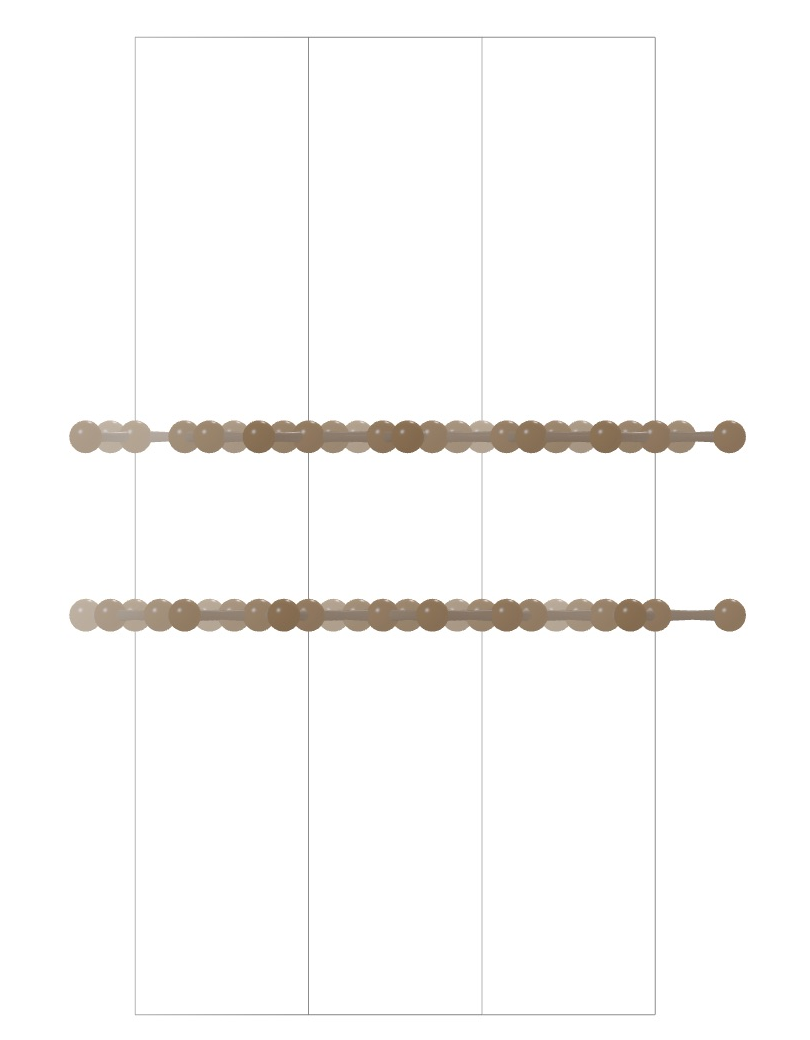
\includegraphics[width=67mm]{publication-assets/crop-a8d161a93e2745b16ef3.png}
\caption{同一模型的侧视。两张原子平面与法向晶胞边界一起显示，便于分辨层间距离和外侧真空。}
\label{fig:online-twist-side}
\end{figure}

随书参考结构的实际匹配角为 $21.786789298^\circ$，与目标角相差约 $2.98\times10^{-7}$ 度，面内应变为 0。检查两层近邻键的方向，也可得到这一相对角度。

精确的角度和匹配信息保存在原生 JSON 的\file{properties}下的\file{moire}部分。用普通文本编辑器打开本例 JSON，搜索\file{achieved_angle_degrees}即可找到实际角；\file{target_angle_degrees}是目标角，\file{angle_error_degrees}是两者的偏差，\file{in_plane_strain}是面内应变。对自己生成的结构，在查看器的\ui{Export file}中选择\ui{Structure file}，再选 JSON 导出。不应选择同一菜单里的\ui{Scene JSON}，后者保存查看场景，不能用来查找上述结构匹配信息。

\subsection{目标角与实际角为什么可能不同}

目标角的输入范围为 $0^\circ$ 到 $60^\circ$。按六方面内晶格的对称关系，工具把实际匹配角表示在 $0^\circ$ 到 $30^\circ$ 之间；比较较大目标角时，也应按这一表示约定查看结果。本节先在这个较小范围内练习，便于直接比较目标值与实际值。

共同周期只能由特定整数关系构成。输入一个任意小数角，并不意味着一定存在大小合适、又完全等于该角的周期胞。本例把目标改成 $22^\circ$，保持其他参数不变，仍然得到 28 位点结构，实际角仍约为 $21.786789298^\circ$，角度偏差约为 $0.213211^\circ$。

这两次构建具有相同的最终几何，却对应不同的目标输入。随书\file{graphene-twist-target22.json}保留了第二次结果，便于比较。报告模型时，应记录实际角，而不是只把参数窗口中输入的目标角写进图题。

\begin{table}[htbp]
\centering
\caption{本组输入下目标角与规模限制的实际对照。}
\begin{tabularx}{\linewidth}{lX}
\toprule
输入变化 & 实际生成结果\\
\midrule
目标 $21.786789^\circ$，上限200 & 28位点，实际约 $21.786789298^\circ$。\\
目标 $22^\circ$，上限200 & 仍为28位点和同一实际角，偏差约 $0.213211^\circ$。\\
目标 $21.786789^\circ$，上限24 & 本例选择4位点、接近 $0^\circ$ 的匹配，未达到原目标。\\
\bottomrule
\end{tabularx}
\end{table}

第三行说明，完成构建与达到目标角是两项不同的检查。28位点的匹配被上限24排除后，工具会在剩余范围内选择结果。构建后，看到数量与预期明显不同，应回到参数和实际角一起核对，再决定是否增大搜索范围。

较小转角通常需要较长的共同周期和更多原子。比较不同转角时，可以先固定层间距与应变要求，再逐步增加允许的模型规模和匹配指数。这样更容易看清新增的搜索范围究竟改善了角度匹配，还是只带来更大的结构。本节约 $21.8^\circ$ 的例子使用较小整数，适合作为操作和周期检查的起点。

\subsection{按研究目的选择组装入口}

\ui{界面建模}菜单把几种组装方式放在一起。选择时，先明确已经知道哪些几何关系，再决定让工具寻找什么。

\begin{table}[htbp]
\centering
\caption{直接插入、层匹配与扭转构建的选择。}
\begin{tabularx}{\linewidth}{lX}
\toprule
入口 & 适合开始的情形\\
\midrule
插入结构 & 两部分的位置已经确定，只需给出相对平移；保留当前宿主晶胞。\\
堆叠异质结构 & 希望比较共同面内晶胞，从允许应变、重复范围与旋转范围中选择候选。\\
扭转莫尔超晶格 & 已有六方单层和目标转角，希望寻找相应的整数共同周期。\\
\bottomrule
\end{tabularx}
\end{table}

在\ui{堆叠异质结构}的候选表中，面积、应变、原子数和旋转角各自回答不同问题。面积与原子数反映计算规模；应变说明原始晶格需要改变多少才能匹配；旋转角说明两层如何相对定向。应变很小的候选也可能很大，面积最小的候选也可能需要较大形变。先比较这些量，再看具体原子排列，选择会更有依据。

本节的扭转命令则先利用六方整数关系确定一组共同周期，再组装两层。它不会要求在同一个窗口中填写\ui{候选序号}。如果希望比较目标 $21.786789^\circ$ 与 $22^\circ$，应分别从两张原始单层构建，分别记录结果，而不是在前一个已完成的双层上再次施加相同命令。

同样，直接旋转屏幕上的观察方向只会改变视角；选择一组原子进行旋转则改变原子位置。两者都不能代替共同晶胞的周期匹配。检查扭转模型时，除观察两层取向，还应显示晶胞边框，沿两个面内方向查看重复后的连接，确认局部图案与整个周期表达的是同一模型。

这组入口用于沿法向叠放的层状界面。构建面内并排相接的异质结时，需另行准备结区的原子排列与边界。

\subsection{进一步建立石墨烯/h-\headinglatin{BN}扭转异质结构}

扭转不只用于同一种材料的双层。前面石墨烯与 h-BN 的零转角匹配，主要展示两种面内晶格常数如何协调；在此基础上，还可以同时引入相对转角。本例仍使用石墨烯作为底层，h-BN 作为上层：石墨烯晶格常数为 $2.46\,\text{\AA}$，h-BN 为 $2.50\,\text{\AA}$。

\begin{steps}
  \item 重新导入\file{twist-graphene-bottom.json}与\file{hBN-layer.json}，分别命名为\file{graphene-bottom}和\file{hBN-top}。不要把前一个已经扭转的双层作为底层。
  \item 激活新的石墨烯单层，在\ui{扭转莫尔超晶格}中将\ui{上层结构}选择为\file{hBN-top}。
  \item 沿用表中的目标角、层间距、总真空、200位点上限与匹配指数6，允许最大面内应变仍设为0.03。
  \item 预览后核对组成应为 $\mathrm{C_{14}B_7N_7}$，共28个位点。上层和底层各有14个位点，但元素组成不同。
  \item 应用并保存为\file{graphene-hBN-twist-21p786789}，再与零转角的\file{graphene-hBN-stacked.json}比较。
\end{steps}

本例实际角同样约为 $21.786789298^\circ$，面内主应变为 0.016，即 1.6\%。h-BN 的面内尺寸被匹配到石墨烯共同晶格，层间距仍为 $3.35\,\text{\AA}$，法向胞高仍为 $18.35\,\text{\AA}$。应变和转角描述的是不同变化：前者调整尺寸，后者改变两层的相对方向。

两种构建命令得到的都是几何模型。研究界面电荷转移、能带对齐或结区性质时，需要在保存的结构上继续建立相应计算，并区分构建输入的层间距与计算后得到的距离。

\subsection{保存扭转模型}

保存项目可以保留输入层、生成结构和后续工作流。单独交换结构时，本组提供 JSON 与 CIF 两种格式：JSON保留面内/法向周期标记、层编号和扭转匹配信息；CIF便于交换晶胞与原子位置。导入本组CIF时，三个方向均按周期处理，莫尔匹配信息需另行保留。继续本章的二维建模比较，优先使用JSON；使用CIF进入其他计算流程时，再按目标方法确认法向边界与真空设置。

\begin{steps}
  \item 为每个结果写清材料、实际角和主要变化，例如“石墨烯双层，实际21.7868度”，不要只保存\file{result}之类的通用名称。
  \item 记录输入层的晶格、目标角与实际角、应变、层间距、总真空、位点数及面内周期。比较表可将这些量各占一列。
  \item 保存项目后重新打开，再检查上下两层的组成和晶胞。导出结构时，保留对应的参数记录，便于解释另一个软件中看到的模型。
  \item 需要重复生成时，以\file{-nojvm}启动MATLAB\regmark{}，配置好工具箱路径后，从随书示例目录运行\file{twist_examples.m}；只检查已保存文件时，运行\file{verify_twist_examples.m}。
\end{steps}

随书结构是用于后续弛豫和电子结构计算的初始模型。比较扭角效应时，采用一致的泛函、赝势、截断能和合适的采样条件，并将计算设置与结构一同保存。


\section{准备 \headinglatin{NEB} 初始路径}

\ui{生成 NEB 路径}需要项目中的初态与终态。两端结构必须具有相同的原子数量、元素排列与晶格，才能使原子一一对应。默认生成 5 个中间构型，并用 IDPP 改善插值中的原子间距。生成后逐幅检查移动轨迹和近距离接触；这些中间结构用于后续路径计算，反应能垒由能量计算确定。

\subsubsection{中间构型怎样分布}

若填写$M$个中间构型，连同两端共有$M+2$个结构。以$j=0,\ldots,M+1$编号。对于非周期模型，或已选定连续周期映像的两端，线性插值的位置关系为
\begin{equation}
  \alpha_j=\frac{j}{M+1},\qquad
  \mathbf r_i^{(j)}=(1-\alpha_j)\mathbf r_i^{(0)}
     +\alpha_j\mathbf r_i^{(M+1)}.
  \label{eq:neb-image-interpolation}
\end{equation}
$i$表示同一个原子在两端对应的序号，$\alpha_j$是无量纲路径参数，位置以\AA 表示。周期结构还要按所用周期边界处理端点位移，不能将同一原子在两个不同周期映像中的坐标直接当作很长的迁移距离。

IDPP进一步使每个构型中的原子对距离接近插值目标：
\begin{equation}
\begin{aligned}
  d_{ik}^{*,(j)}&=(1-\alpha_j)d_{ik}^{(0)}
                      +\alpha_j d_{ik}^{(M+1)},\\
  E_{\mathrm{IDPP}}^{(j)}&=
    \sum_{i<k}\frac{\bigl(d_{ik}^{(j)}-d_{ik}^{*,(j)}\bigr)^2}
                         {\bigl(d_{ik}^{(j)}\bigr)^4}.
\end{aligned}
\label{eq:idpp-pair-objective}
\end{equation}
其中$i,k$为原子序号，$j$为构型序号；$d_{ik}^{(j)}$是当前原子对距离，$d_{ik}^{*,(j)}$是对应的目标距离。分母使过短的原子间距受到较强惩罚，因此IDPP往往能改善线性插值中的碰撞。上式给出单个构型的原子对目标；路径优化还会考虑相邻构型之间的联系。

$E_{\mathrm{IDPP}}$是几何插值的辅助目标，其值用于评价路径几何；反应能垒需由后续能量计算确定。窗口中的\ui{IDPP力收敛阈值}用于这一步辅助优化，与电子结构计算中的原子力阈值分别设置。$M=5$时，路径参数依次为$0,1/6,2/6,\ldots,1$；本例的00至06正好对应七个结构。


\subsection{练习：检查五个中间构型}
\index{NEB@NEB 路径}

随书\file{neb-exchange/initial.json}与\file{final.json}提供一个容易看清原子对应的几何例子。两个带有不同标签的 H 原子在 $10\,\text{\AA}$ 的非周期立方盒中交换位置：初态坐标为 $(2,5,5)$ 和 $(8,5,5)\,\text{\AA}$，终态将这两个位置对调。这里研究的是插值如何避开原子重合，不把它作为氢分子反应。

\begin{steps}
  \item 把两份端点文件导入同一项目，分别命名为\file{initial}与\file{final}。核对两端原子顺序与标签一致，再激活初态。
  \item 在\ui{晶体建模}的\ui{表面与界面}区域，打开\ui{界面建模}，选择\ui{生成 NEB 路径}。在\ui{NEB 终态结构}下拉菜单中选择项目内的终态\literalinput{final}。
  \item \ui{NEB 中间构型数}设为 5，\ui{IDPP 最大优化步数}保持 200，\ui{IDPP 力收敛阈值}保持 0.1。预览并应用后，在项目浏览器的结构分组中找到\literalinput{NEB image 00}至\literalinput{NEB image 06}，依次打开。这7个结构包含两端和5个中间构型。
  \item 依序观察原子标签和两点距离。两端应保持原坐标，中间构型则绕开原来会重合的位置。保存当前项目，即可同时保留两端输入和这7个结果；需要单独交换某幅时，再导出相应结构。
\end{steps}

若直接作直线插值，两个原子会在中间一幅重合。参考路径的 IDPP 优化经 82 次迭代达到阈值，全路径最短的两点距离约为 $3.5755\,\text{\AA}$，中间一幅约为 $3.7380\,\text{\AA}$。\file{image-00.json}至\file{image-06.json}保存全部路径结构，便于逐幅比较。IDPP 报告中的目标值和数值力用于评价初始路径，不是后续电子结构计算的能量和原子力。

图~\ref{fig:neb-idpp}~把这些坐标与直线插值放在一起比较。左图中的线段连接已生成的结构，右图给出相应两点距离；沿图号检查，可以同时确认两端不变和中间接触改善。

\begin{figure}[H]
\centering
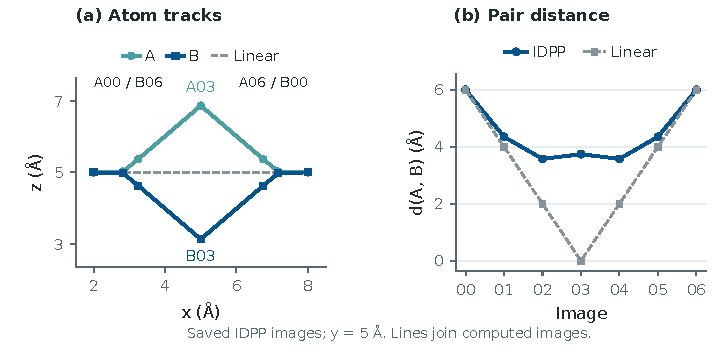
\includegraphics[width=\linewidth]{publication-assets/vector-79e6f35b7afec0271551.pdf}
\caption{两个原子交换位置的 IDPP 参考路径。左：固定 $y=5\,\text{\AA}$ 时的 $x$--$z$ 轨迹，A00/B06 等标签标出端点对应；右：00至06各构型的两点距离。灰色虚线为直线插值，03为中间构型。}
\label{fig:neb-idpp}
\end{figure}

\section{示例：建立低维模型}\label{sec:nanostructure-examples}
\index{Namidai@纳米带}\index{Namiguan@纳米管}\index{Namixian@纳米线}

把片层裁成带，或沿一个方向卷成管，会改变结构的边界和周期。纳米带在宽度方向出现边缘，只沿长度方向重复；纳米管沿轴向重复，另外两个方向留出真空。由块体截取的纳米线也只有一个周期方向；有限团簇则在三个方向都不重复。

本节先用一份小的石墨烯原胞建立24位点纳米带和32位点纳米管，再从面心立方铜建立纳米线、有限团簇和球形空洞。每个结果都配有原生JSON与CIF文件，可一边构建，一边与随书结果比较。

\subsection{准备六十度石墨烯原胞}

随书\file{nano-graphene-60.json}含两个C位点，面内两个晶格矢量长度均为 $2.46\,\text{\AA}$，夹角 $60^\circ$，法向盒高 $15\,\text{\AA}$；两个面内方向周期，法向非周期。它与前面的\file{graphene-layer.json}表示同一张石墨烯，区别是晶格基底的选取。

若从前面的 $120^\circ$ 原胞出发，可保留 $\mathbf a$，将第二个矢量换成 $\mathbf a+\mathbf b$。新矢量仍长 $2.46\,\text{\AA}$，但与 $\mathbf a$ 的夹角成为 $60^\circ$。这次整数换基的行列式为1，因此不会扩大模型，仍有两个独立位点。本节的带和管均使用这份 $60^\circ$ 输入。

\begin{steps}
  \item 将\file{nano-graphene-60.json}导入项目，命名为\file{nano-graphene}，打开三维文档，检查两个独立位点、等长的面内晶格和 $60^\circ$ 夹角。
  \item 如希望自己换基，另行导入原始\file{graphene-layer.json}并激活。在\ui{晶体建模}\,$\rightarrow$\,\ui{超胞与晶格}中打开\ui{构建超胞}。
  \item 在\ui{超胞倍率或变换矩阵}文本框中输入\literalinput{1 0 0; 1 1 0; 0 0 1}。这是三行整数矩阵，分号用于分行；与编辑晶格窗口的逐格表格不同。
  \item 预览后核对位点数仍为2，晶胞体积保持不变，面内夹角变为 $60^\circ$。应用后另存为能说明基底的名称，不覆盖原来的 $120^\circ$ 单层。
  \item 为纳米带与纳米管分别保留一份输入。每次构建都从单层开始，不能在已经裁成带的结果上继续执行卷管而当作同一个例子。
\end{steps}

两种基底的晶胞边框看起来不同，但原材料的周期几何相同。使用本节命令时，先核对输入文件与基底，再比较位点数和尺寸；只抄写宽度或手性指数，不足以确定同一个构建过程。

\subsection{裁出一条扶手椅边石墨烯纳米带}

纳米带的宽度和轴向长度按重复单元数填写；真空以\AA 为单位。\ui{armchair}与\ui{zigzag}描述两种不同的边缘排列，不是两个相机方向。这里选择扶手椅边，先检查边缘上的碳原子怎样成对排列，再看沿带长方向的周期连接。

\begin{table}[htbp]
\centering\small
\caption{24位点扶手椅边纳米带的参数。}
\begin{tabularx}{\linewidth}{lX}
\toprule
字段 & 本例输入\\
\midrule
宽度方向重复单元数 & 3，无量纲整数。\\
轴向重复单元数 & 2，无量纲整数。\\
边缘类型 & 选择\ui{armchair}。\\
真空层厚度（Å） & 5；本工具在两个非周期方向的两侧分别留出该空白。\\
最大原子数 & 500；是构建规模上限，不是要求最终有500个位点。\\
\bottomrule
\end{tabularx}
\end{table}

\begin{steps}
  \item 激活准备好的\file{nano-graphene}单层。从\ui{晶体建模}的\ui{纳米结构}菜单打开\ui{截取纳米带}。
  \item 按表填写参数。宽度3不是 $3\,\text{\AA}$；轴向2也不是 $2\,\text{\AA}$。
  \item 单击\ui{预览}，显示晶胞边框。沿片层法向查看两条边，转到侧面确认模型仍是一张平带。
  \item 检查独立位点数为24，所有原子均为C。沿周期方向查看接续，不能把靠近晶胞两端的同一周期网络看成两段断开的分子。
  \item 应用后命名为\file{graphene-armchair-w3-l2}，保存项目，并与随书同名JSON比较。原单层仍需单独保留。
\end{steps}

本例输出在全局 $y$ 方向周期，原生周期标记为\literalinput{false true false}。三个胞长约为 $16.15$、$8.521690$、$10.00\,\text{\AA}$。其中沿带长的周期为 $8.521690\,\text{\AA}$；原子在宽度方向的实际跨度为 $6.15\,\text{\AA}$，再加两侧各 $5\,\text{\AA}$ 空白，得到 $16.15\,\text{\AA}$ 的盒宽。平片本身没有法向厚度，所以该方向的盒长为 $10\,\text{\AA}$。

未钝化的24个C原子中，以 $1.65\,\text{\AA}$ 为近邻检查界限，有16个原子连接三个近邻，8个边缘原子连接两个近邻；最短周期原子间距约为 $1.420282\,\text{\AA}$。这个界限用于核对这组碳模型，并不是所有元素的通用成键距离。若要研究氢钝化边缘，应另存未钝化模型，再按目标边缘配位添加氢并检查组成。

\subsection{把石墨烯卷成一根小纳米管}

卷曲前先确定平面中哪一条矢量将成为管的圆周。帮助信息中的几何关系为
\begin{equation}
  \mathbf C_h=n\mathbf a_1+m\mathbf a_2,
  \qquad R=\frac{\|\mathbf C_h\|}{2\pi}.
  \label{eq:nanotube-circumference-radius}
\end{equation}
$\mathbf a_1,\mathbf a_2$是输入片层的面内晶格矢量，单位为\AA；$n,m$是无量纲手性指数，$\mathbf C_h$是手性矢量，$R$为初始管半径。圆周长度取两个基矢线性组合的模。等长、夹角$60^\circ$的面内基矢给出$\|\mathbf C_h\|=a\sqrt{n^2+nm+m^2}$；换用其他基底时，应回到式\eqref{eq:nanotube-circumference-radius}计算。本节沿用已整理好的$60^\circ$输入；不同基底中的同一组$(n,m)$不应直接视为同一卷曲方向。

\begin{figure}[htbp]
\centering
\begin{tikzpicture}[x=1mm,y=1mm,font=\sffamily\small,>=stealth]
  \node[text=brand] at (26,54) {平面中的卷曲方向};
  \foreach \j in {0,1,2,3} {
    \draw[teal!55] ({6+4*\j},{10+7*\j}) -- ({38+4*\j},{10+7*\j});
    \foreach \i in {0,1,2,3,4} {
      \fill[brand] ({6+8*\i+4*\j},{10+7*\j}) circle (.8);
    }
  }
  \foreach \i in {0,1,2,3,4}
    \draw[teal!55] ({6+8*\i},10) -- ({18+8*\i},31);
  \draw[->,brand,line width=.9pt] (6,10) -- (38,10)
    node[midway,below=3pt] {$\mathbf C_h=4\mathbf a_1$};
  \draw[->,muted] (6,10) -- (14,10) node[above] {$\mathbf a_1$};
  \draw[->,muted] (6,10) -- (10,17) node[left] {$\mathbf a_2$};
  \draw[->,teal,line width=.8pt] (57,24) -- (69,24);
  \node[text=muted,font=\sffamily\footnotesize] at (63,32) {卷合};
  \node[text=brand] at (95,54) {圆周长度不变};
  \fill[paleblue] (81,10) rectangle (109,39);
  \draw[brand,line width=.8pt] (81,10) -- (81,39);
  \draw[brand,line width=.8pt] (109,10) -- (109,39);
  \draw[brand,fill=paleblue,line width=.8pt] (95,39) ellipse (14 and 5);
  \draw[brand,line width=.8pt] (81,10) arc[start angle=180,end angle=360,x radius=14mm,y radius=5mm];
  \draw[brand,densely dashed] (109,10) arc[start angle=0,end angle=180,x radius=14mm,y radius=5mm];
  \draw[->,muted] (95,39) -- (109,39) node[midway,above] {$R$};
  \draw[->,teal] (115,10) -- (115,43) node[above] {管轴};
  \node[align=center,font=\sffamily\footnotesize] at (95,-1) {$\|\mathbf C_h\|=2\pi R$};
\end{tikzpicture}
\caption{手性矢量与管半径的关系（示意）。左图的点表示晶格平移点，以$(4,0)$标出卷成一周的平面方向；右图表示卷曲后圆周与半径的几何关系。}
\label{fig:nanotube-chiral-geometry}
\end{figure}


手性指数 $(n,m)$ 指定卷成圆周的晶格方向，轴向重复数决定沿管轴保留多少个平移周期。本例使用 $(4,0)$，管半径较小，便于观察卷曲、接缝与周期。稳定半径需在几何弛豫后确定。

\begin{steps}
  \item 回到原始\file{nano-graphene-60.json}，另开一份单层文档并激活。不要使用刚生成的纳米带。
  \item 在\ui{纳米结构}菜单选择\ui{生成纳米管}。在\ui{手性指数（n m）}的两个数值框中分别填4与0。
  \item \ui{轴向重复单元数}设为2，\ui{真空层厚度（Å）}设为6，\ui{最大原子数}设为500。
  \item 预览后沿管轴观察环形截面，再从侧面检查管身。转动相机查看卷合位置，并核对轴向两端能按周期相接。
  \item 检查模型共有32个C位点。应用后保存为\file{graphene-tube-4-0-l2}，保留单层输入和纳米管结果。
\end{steps}

本例沿全局 $z$ 方向周期，周期标记为\literalinput{false false true}。由卷曲圆周得到的半径为
\[
 R=\frac{4\times2.46}{2\pi}\,\text{\AA}\approx1.566085\,\text{\AA}.
\]
两个横向胞长均约为 $15.132169\,\text{\AA}$，等于管直径加两侧各 $6\,\text{\AA}$ 真空；轴向胞长约为 $8.521690\,\text{\AA}$。本工具的横向真空与扭转双层窗口中的\ui{总真空层厚度}含义不同，比较盒长时应按各命令的定义计算。

对保存坐标作周期近邻检查，32个位点均有三个距离小于 $1.65\,\text{\AA}$ 的近邻，最短间距约为 $1.393202\,\text{\AA}$。平片卷成很小的圆周后，两点之间的直线距离会与平面上的距离不同。因此，不必要求卷管后的全部C--C直线距离仍恰好等于平片的 $1.420282\,\text{\AA}$；应同时检查半径、接缝、近邻与周期，后续几何弛豫另行进行。

\subsection{从管口与侧面阅读纳米管}

已构建的纳米管也可以直接从随书\file{graphene-tube-4-0-l2.json}导入。这样可以先熟悉观察方法，再回到参数窗口比较不同的手性指数。初次取景保持\ui{Input cell}与\ui{1 × 1 × 1}，使画面对应保存的一个模型周期。

\begin{steps}
  \item 在\ui{主页 → 结构 → 从文件导入结构}中选择该JSON；在线版先上传，再从云文件导入。打开结构文档，确认元素为C，模型摘要为32个位点。
  \item 在视图工具栏单击\ui{c}，其提示为\ui{View along c axis}。本例管轴与$c$平行，因此现在从管口看向管内；观察碳原子围成的环和中央空心区域。
  \item 单击\ui{a}或\ui{b}转到侧面。保持相同缩放，检查管身沿轴向延伸，六元环在曲面上的排列仍可辨认。若球体遮住连接，在\ui{Viewer settings → Style}中适度减小\ui{Atom scale}，再查看局部。
  \item 在\ui{Visibility}中显示\ui{Unit cell}，把细长的管身与横向真空盒比较。需要看清单个周期的原子时，可先隐藏\ui{Boundary image atoms}；检查两端接续时再显示边界映像。
  \item 在\ui{Scientific scene → Repeat cell}中只把\ui{c}设为2，观察轴向两段怎样接上。看完使用\ui{Reset to 1 × 1 × 1}恢复，最后单击\ui{Reset camera}重新取全景。
  \item 分别导出管口和侧面图片，记录两图来自同一32位点结构，并注明$(4,0)$、轴向两个重复单元及原始JSON文件名。
\end{steps}

沿管轴看见“孔”，说明当前坐标围成了管形；侧面和重复显示则帮助确认它沿轴向周期延伸。显示重复没有把输入改成更大的计算超胞。边界附近增加的球体也属于场景映像，模型独立位点数仍应按原始结构读取。以这两种取向共同说明形态，比只留一张斜视图更容易辨认管径、管长与周期。

\begin{figure}[!htb]
\centering
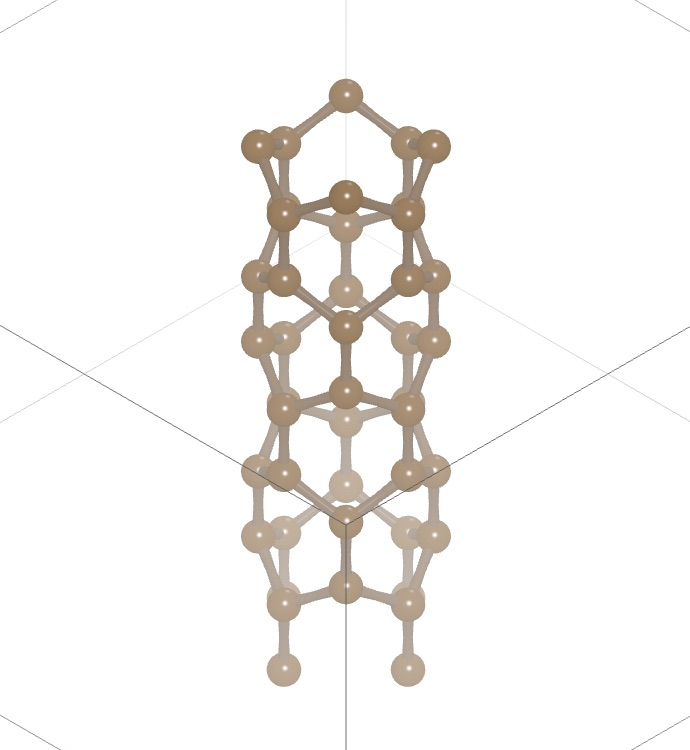
\includegraphics[width=.47\linewidth]{publication-assets/revision-nanotube-perspective.png}\hfill
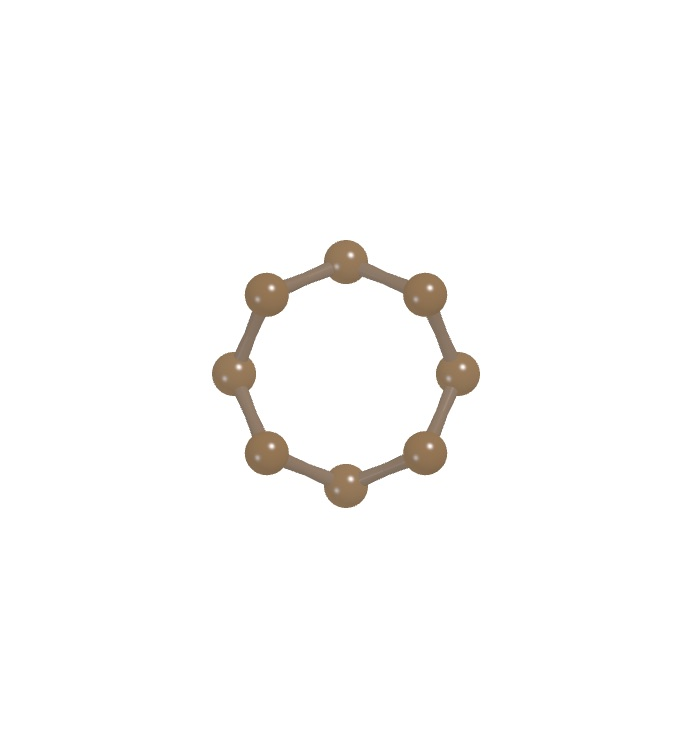
\includegraphics[width=.47\linewidth]{publication-assets/revision-nanotube-axis-c.png}
\caption{同一32位点碳纳米管的三维视图。左：从侧面检查曲面的碳网络和轴向连接；右：沿管口方向观察中央空心区域。显示中包含周期边界映像，独立位点数保持32。}
\label{fig:nanotube-live}
\end{figure}

\FloatBarrier
\subsection{从铜晶体截取纳米线}

铜例子使用随书\file{nano-Cu-fcc-input.json}，与\file{Cu-fcc.cif}来自相同的四位点面心立方晶胞，晶格常数为 $3.61\,\text{\AA}$。纳米线保留一个晶格方向的平移周期，横截面则按给定半径截取。截取球或圆柱时，原子不是连续分布的介质；实际最外原子的跨度不一定等于两倍输入半径。

周期方向指数$[u\,v\,w]$通过实空间晶格给出线轴方向：
\begin{equation}
  \mathbf t=u\mathbf a+v\mathbf b+w\mathbf c.
  \label{eq:nanowire-lattice-direction}
\end{equation}
$u,v,w$为无量纲整数，$\mathbf t$与晶格矢量使用相同的长度单位。构建时取与$\mathbf t$平行的轴，再以给定半径保留横截面内的原子；轴向周期长度以输出晶胞为准。

\begin{table}[htbp]
\centering
\caption{晶格方向指标与晶面指标的区别。}
\begin{tabularx}{\linewidth}{lX}
\toprule
输入 & 对应的几何关系与用途\\
\midrule
$[u\,v\,w]$方向 & 由实空间的$\mathbf a,\mathbf b,\mathbf c$组合得到，用于纳米线轴向等方向选择。\\
$(hkl)$晶面 & 由倒格矢组合得到法向，见式\eqref{eq:surface-miller-normal}，用于表面切割。\\
\bottomrule
\end{tabularx}
\end{table}

在立方晶胞中，同一组三个整数给出的方向与同指数晶面的法向平行；在一般斜晶胞中并非如此。填写前先看窗口要求的是方向还是晶面，再从轴向和侧向检查预览。

\begin{steps}
  \item 导入铜输入并激活，在\ui{纳米结构}中打开\ui{截取纳米线}。
  \item 在\ui{周期方向指数（u v w）}的三个框中分别填0、0、1；半径设为 $3\,\text{\AA}$，轴向重复单元数设为2，真空层厚度设为 $4\,\text{\AA}$，最大原子数设为2000。
  \item 预览时沿线轴观察截面，确认原子位于选定圆柱内。再从侧面看轴向接续，核对共有24个Cu位点。
  \item 应用并保存为\file{Cu-wire-001-r3-l2}。改变半径或方向时，从原始铜晶体重新开始，避免把有限横截面再次当成块体截取。
\end{steps}

结果沿 $z$ 轴周期，周期标记为\literalinput{false false true}，轴向胞长为 $7.22\,\text{\AA}$。两个横向原子跨度均为 $5.415\,\text{\AA}$，加上两侧各 $4\,\text{\AA}$ 的空白后，两个横向盒长均为 $13.415\,\text{\AA}$。最短周期近邻距离约 $2.552655\,\text{\AA}$，与输入面心立方铜的最近邻距离相同。

最大原子数同时约束构建时需要的母超胞规模。本例采用2000；若上限过小，按提示检查母超胞的规模后再调整。

\begin{figure}[!htb]
\centering
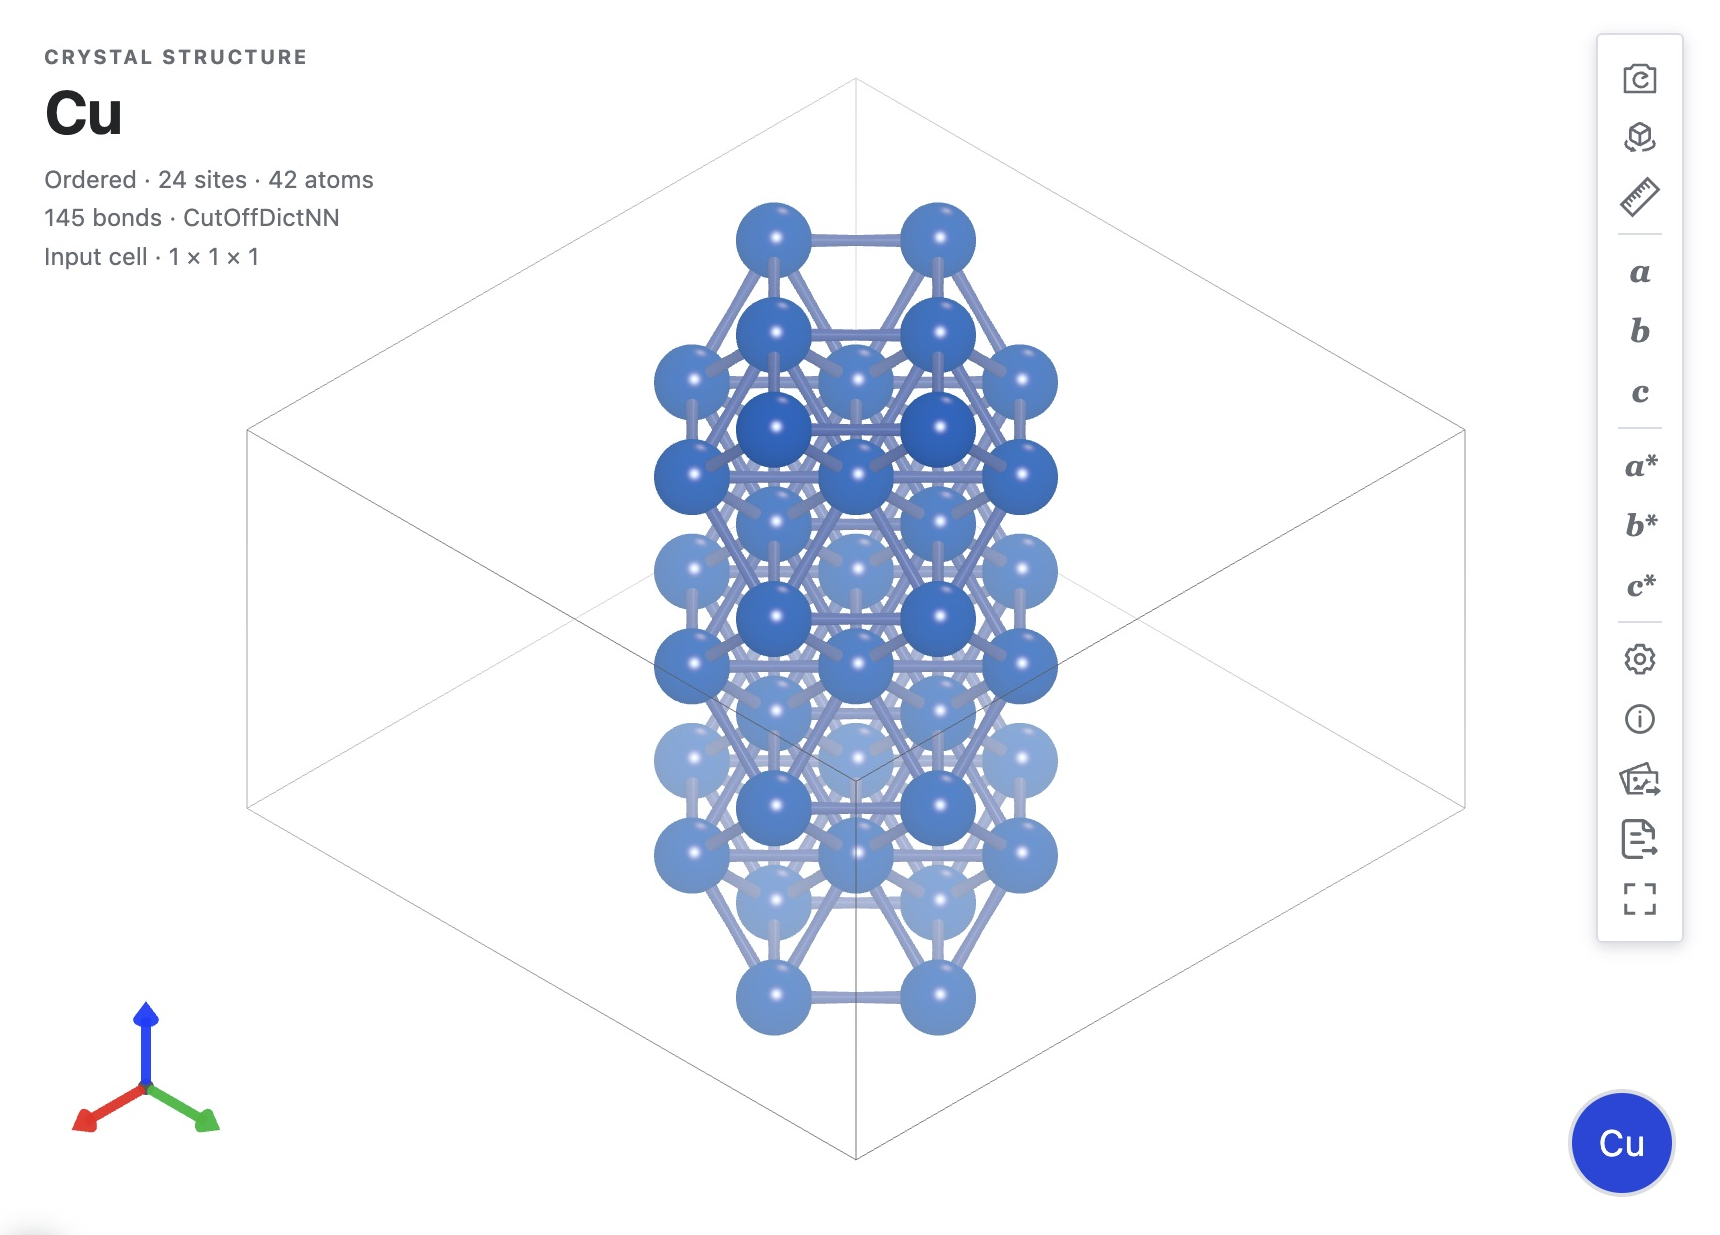
\includegraphics[width=\linewidth]{publication-assets/revision-nanowire-perspective.png}
\caption{随书24位点铜纳米线的实际显示。查看器补出周期边界原子以展示轴向连接，横向的空白属于真空区域。}
\label{fig:nanowire-live}
\end{figure}

\FloatBarrier
\subsection{检查纳米线的截面与轴向}

打开随书\file{Cu-wire-001-r3-l2.json}，即可检查已经截取的24位点铜纳米线。它与纳米管都沿$c$方向周期。纳米管由单层卷成空心圆周；铜纳米线保留圆柱范围内的晶体原子，横截面内部也有原子。

\begin{steps}
  \item 导入JSON并打开三维文档，保持\ui{Input cell}。核对元素为Cu、独立位点为24。
  \item 单击视图工具栏的\ui{c}沿线轴观察截面。原子排列在离散的晶格位置上，轮廓可以呈阶梯状，不必形成光滑圆边。
  \item 单击\ui{a}或\ui{b}看侧面，打开\ui{Unit cell}。用轴向$7.22\,\text{\AA}$与横向$13.415\,\text{\AA}$的盒长解释取景：沿轴向是重复周期，横向大盒用于容纳有限截面与真空。
  \item 清除无关选择，稍微旋转为同时看见截面和侧面的斜视图。保留晶胞边框与方位标记，检查没有原子被视图边缘裁掉。
  \item 按需要将\ui{Repeat cell}的\ui{c}设为2查看接续，随后恢复一个周期。保存项目与结构；导出图片时在图注记录$[001]$方向、输入截取半径$3\,\text{\AA}$和24个位点。
\end{steps}

输入半径决定保留哪些晶格位置，图中最外原子的跨度则由实际保留的离散位置决定。本例横向跨度$5.415\,\text{\AA}$小于直径$6\,\text{\AA}$，与截取规则一致。后续结构优化及电子性质分析可使用相应计算工作流。

\subsection{截取一个有限铜团簇}
\index{Liangzidian@量子点}

\ui{量子点 / 纳米空洞}的\ui{量子点}模式保留球内原子，建立三个方向均不周期的有限结构。本例用13位点铜团簇观察有限边界与周期块体的区别，保存后可继续安排相应的电子结构计算。

\begin{steps}
  \item 重新激活四位点铜输入，从\ui{纳米结构}打开\ui{量子点 / 纳米空洞}。
  \item 处理方式选择\ui{量子点}，半径填 $3\,\text{\AA}$，真空层厚度填 $4\,\text{\AA}$，最大原子数设为2000。
  \item 预览后旋转观察，确认没有一条方向继续连接成无限原子链。检查共有13个Cu位点。
  \item 应用并命名为\file{Cu-dot-r3}，保存项目和结构。
\end{steps}

本例的三个胞长均约为 $11.61\,\text{\AA}$，原子在各方向的跨度均为 $3.61\,\text{\AA}$，三向周期标记均为false。最短原子间距约 $2.552655\,\text{\AA}$。按 $2.8\,\text{\AA}$ 的近邻界限检查，中心原子有12个近邻，其余12个表面原子各有5个近邻。这一初始团簇从面心立方排列直接裁取，稳定构型需进一步优化。

\subsection{在周期铜中挖出球形空洞}
\index{Namikongdong@纳米空洞}

空洞模式保留球外宿主和原周期盒；它与保留球内原子的量子点模式正好相反。先建立足够大的宿主，可以避免只从很小晶胞中删去大部分甚至全部原子。

\begin{steps}
  \item 导入随书\file{Cu-void-host-2x2x2.json}，或从四位点铜输入通过\ui{构建超胞}建立 $2\times2\times2$ 宿主。应有32个Cu位点，三个胞长均为 $7.22\,\text{\AA}$。
  \item 激活这份宿主，打开\ui{量子点 / 纳米空洞}，处理方式选择\ui{纳米空洞}，半径设为 $2.7\,\text{\AA}$。空洞模式不需要为有限团簇增加外部真空。
  \item 预览并显示晶胞边框。空洞中心固定在宿主的分数坐标 \((0.5,0.5,0.5)\)，应检查晶胞中央的原子被移除，而外围周期宿主仍保留。
  \item 核对本例移除13个原子，剩余19个Cu位点；晶格仍为 $7.22\,\text{\AA}$ 的立方胞，三个方向继续周期。
  \item 应用后另存为\file{Cu-void-r2p7}，保留完整32位点宿主，便于以后改变半径或比较缺陷。
\end{steps}

剩余原子距空洞中心的最短周期距离为 $3.61\,\text{\AA}$。这个值大于输入半径 $2.7\,\text{\AA}$，反映了晶格上可保留的位置是离散的，不表示半径字段失效。剩余宿主的最短原子间距仍约 $2.552655\,\text{\AA}$。保存时同时记录“输入删除球半径”和“剩余最近原子距中心”，会比只给一张透视图更清楚。

\subsection{检查周期并保存配套文件}

每个例子的原生JSON保留当前晶格、坐标、周期标记及相应构建信息；CIF用于交换晶胞和原子几何。导入本组CIF时，三个方向均按周期处理。继续低维建模并保留本节的周期方向时，应使用JSON。

\begin{table}[htbp]
\centering\small
\caption{随书纳米结构的位点数与原生周期。}
\begin{tabularx}{\linewidth}{lX}
\toprule
结果 & 实际模型与主要检查值\\
\midrule
石墨烯纳米带 & 24C；仅$y$周期；轴向 $8.521690\,\text{\AA}$。\\
$(4,0)$纳米管 & 32C；仅$z$周期；半径 $1.566085\,\text{\AA}$。\\
铜纳米线 & 24Cu；仅$z$周期；轴向 $7.22\,\text{\AA}$。\\
铜团簇 & 13Cu；三个方向非周期；盒长各 $11.61\,\text{\AA}$。\\
带空洞的铜 & 19Cu；三个方向周期；32位点宿主中移除13个。\\
\bottomrule
\end{tabularx}
\end{table}

\begin{steps}
  \item 先保存项目，确认输入结构和派生结果具有不同名称。
  \item 如需单独结构文件，在查看器的\ui{Export file}\,$\rightarrow$\,\ui{Structure file}中选JSON，保留模型信息；几何交换可另存CIF。这里不要选择用于显示场景的\ui{Scene JSON}。
  \item 重新打开保存的结构，检查位点数、晶胞和周期方向；再检查边缘、卷合处或球形裁切边界的近邻。
  \item 需要重新生成这组结构时，以\file{-nojvm}启动MATLAB\regmark{}，配置好工具箱路径后，从随书示例目录运行\file{nano_examples.m}。\file{verify_nano_examples.m}用于检查已有结构。
\end{steps}

本节提供未钝化的初始模型，可根据材料与边界需要继续钝化、弛豫和电子结构计算。将模型接入工作流时，保存构建参数与计算参数，并确认工作流引用所需的结构。


\section{示例：建立高分子链}
\index{Gaofenzi@高分子}

\subsection{理解重复单元}

高分子建模从重复单元开始。PE、PP、PS、PEO、PPO 等内置单元可以直接调用；用户重复单元则需要明确头原子、尾原子和连接时移去的原子。头尾定义决定相邻单元如何连接，因此保存重复单元前，应先检查单体拓扑。

均聚物只使用一种重复单元，嵌段共聚物把不同单元组成连续段，无规共聚物则按组成和随机规则生成序列。链序列与空间构象是两类参数：相同的 PE/PP 序列，可以采用伸展、折线或无规线团初始构象。种子用于重现相同的随机构建条件。

\subsection{\headinglatin{PEO--PPO--PEO} 嵌段}

\begin{steps}
  \item 激活分子文档，在顶部\ui{分子建模}的\ui{软物质}区域打开\ui{聚合物建模}，选择\ui{构建嵌段共聚物}。
  \item 在\ui{嵌段重复单元}文本框中输入 \literalinput{PEO PPO PEO}，在\ui{嵌段长度}文本框中输入 \literalinput{3 4 3}，均用空格分隔各项。完整嵌段超单元重复次数设为 1，链数设为 1。
  \item 种子设为 8，\ui{初始构象}下拉菜单先选择\ui{伸展}，首尾端基文本框保持 \file{none}。
  \item 查看预计原子数，预览并应用。检查总共有 10 个重复单元，其中 PEO 合计 6 个，PPO 为 4 个。
  \item 从整体观察链序列，再放大查看两个嵌段交界处的连接。保存为能够表达序列的名称，例如 \file{PEO3-PPO4-PEO3}。
\end{steps}

随书\file{PEO3-PPO4-PEO3.json}由上述参数生成，组成为 $\mathrm{C_{24}H_{50}O_{10}}$，共 84 个原子、83 条键。10 个重复单元连成一条链，相邻单元之间有 9 条连接。虽然端基输入为\file{none}，链两端尚未满足的价键仍由氢补足；核对分子式时应把这些氢计入。

% 插入第8章PEO3–PPO4–PEO3组成段后；本片段不自动修改第8章。
% 全部引用Online原生截图，以独立LaTeX矩形裁切排版，不修改像素。
\begin{figure}[H]
\centering
% 100%浏览器图的核心参数(980,580,2040,1030)，1060×450；105mm约256ppi。
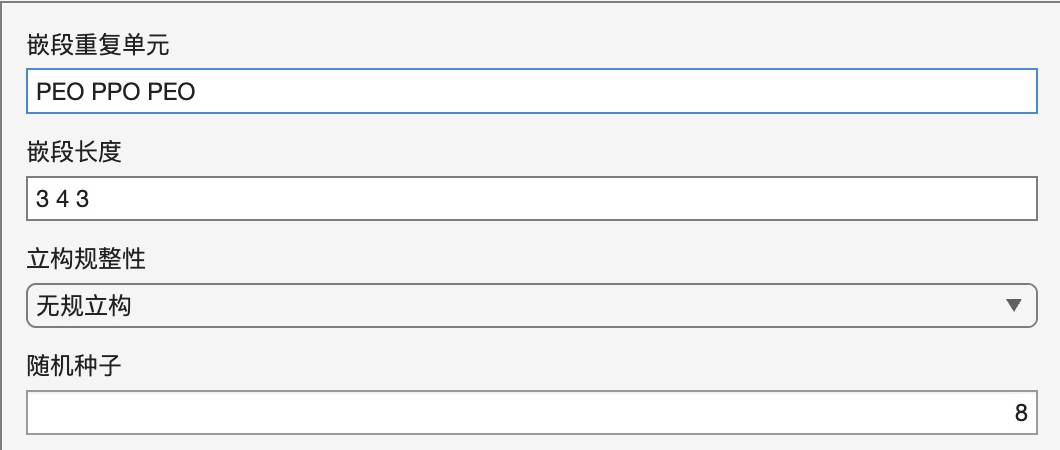
\includegraphics[width=105mm]{publication-assets/crop-3d7aab6f859860340b2f.png}
\par\vspace{3mm}
% 125%浏览器图中下部完整字段(845,710,2175,1535)，1330×825；122mm约277ppi。
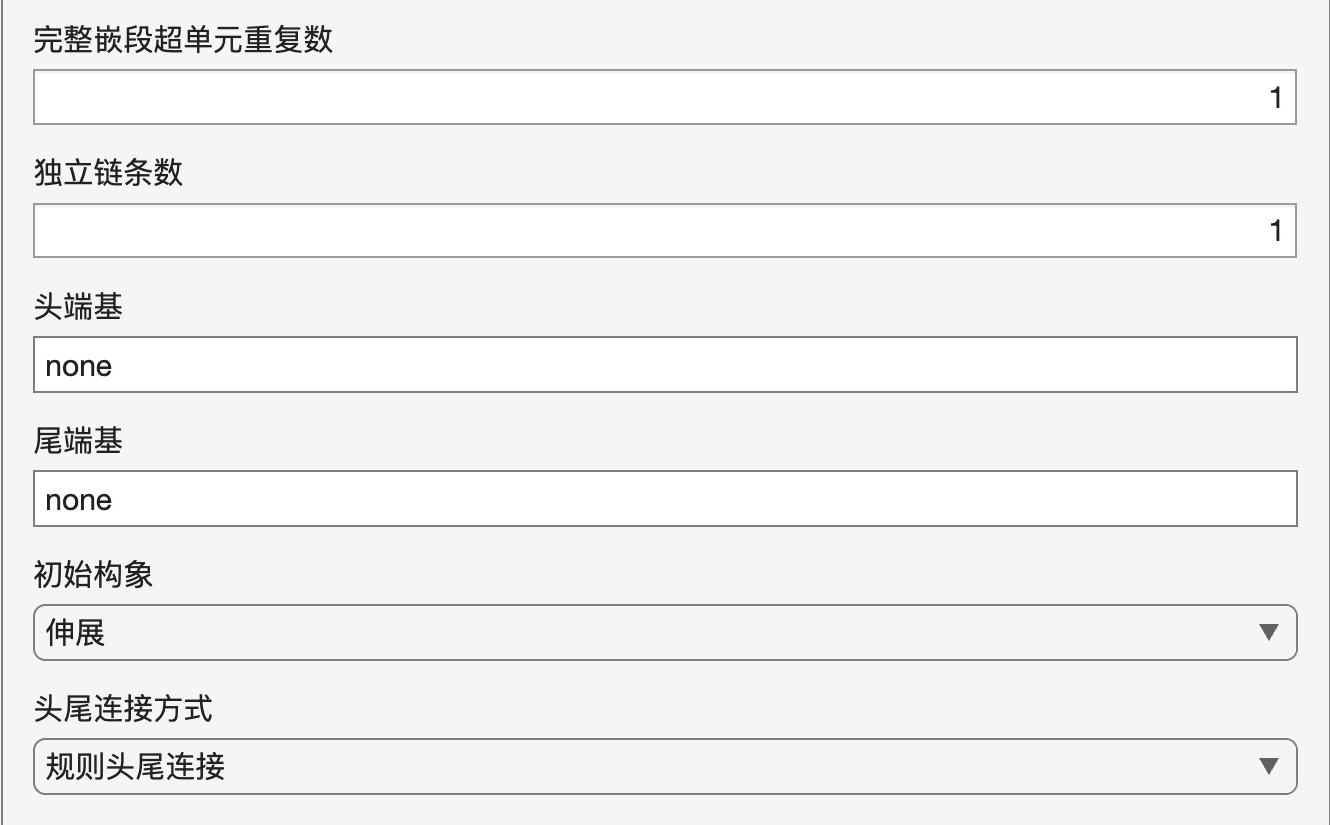
\includegraphics[width=\linewidth]{publication-assets/crop-14436d05d0623e7cdc6f.png}
\caption{构建PEO--PPO--PEO嵌段链的参数。上方输入\literalinput{PEO PPO PEO}、\literalinput{3 4 3}和种子8；下方设为重复1次、1条链、首尾端基均为\file{none}，初始构象为伸展，采用规则头尾连接。}
\label{fig:polymer-block-parameters}
\end{figure}

\begin{figure}[H]
\centering
% 完整链(165,900,2860,1150)，2695×250；122mm约561ppi。
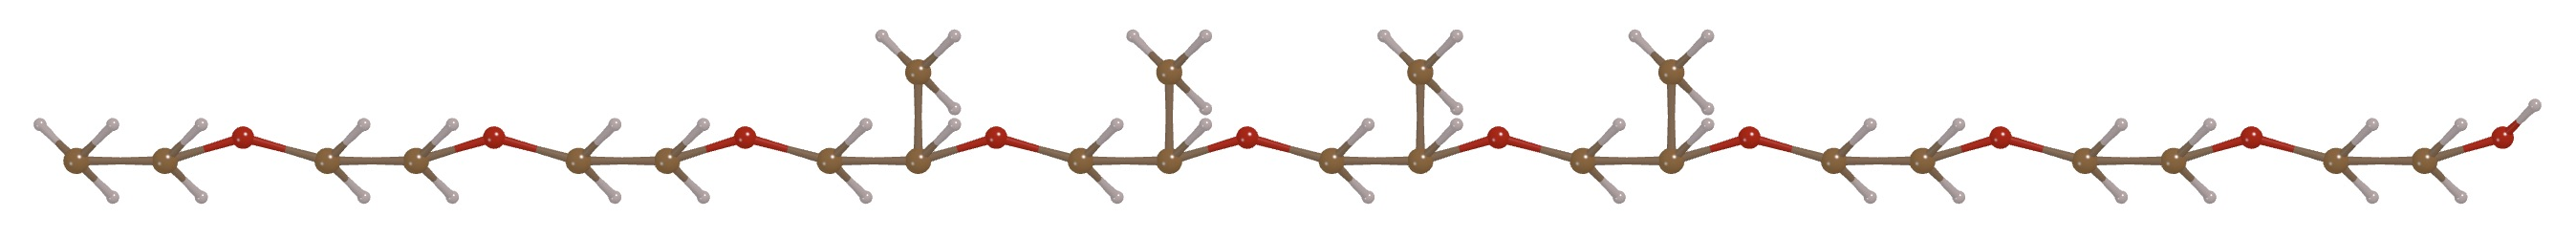
\includegraphics[width=\linewidth]{publication-assets/crop-7684a8a790954b6a1954.png}
\par\vspace{3mm}
\begin{minipage}[t]{40mm}
\vspace{0pt}
% 实际组成摘要(40,330,440,560)，400×230；40mm约254ppi。
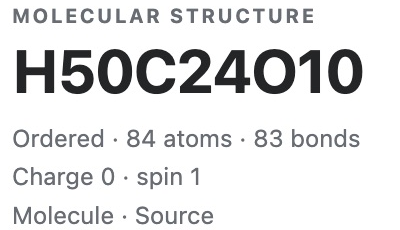
\includegraphics[width=\linewidth]{publication-assets/crop-c77f26280735587ce6a4.png}
\end{minipage}\hfill
\begin{minipage}[t]{80mm}
\vspace{0pt}
% 中部带四个甲基侧支的PPO局部(1000,900,2080,1150)，1080×250；80mm约343ppi。
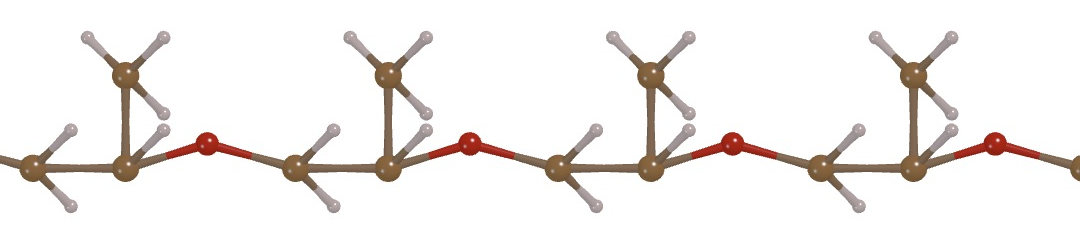
\includegraphics[width=\linewidth]{publication-assets/crop-71a6b6056b817444ef97.png}
\end{minipage}
\caption{应用上述参数后得到的嵌段链初始结构。上方显示整条链；下方左侧摘要为$\mathrm{C_{24}H_{50}O_{10}}$、84个原子和83条连接，右侧放大中部PPO段的四个甲基侧支。}
\label{fig:polymer-block-model}
\end{figure}


\subsection{精确组成的无规链}

另建一个分子文档，选择\ui{构建无规共聚物}，重复单元为 PE、PP，摩尔分数为 0.3、0.7，重复总数为 20，启用精确组成，种子设为 91。此时组成目标是 6 个 PE 和 14 个 PP 单元；它们在链上的具体排列由生成规则和种子确定。

反应性比用于无规序列的终端模型，本例在相应文本框中保持\literalinput{1 1}，初始构象选择\ui{伸展}，\ui{立构规整性}选择\ui{间规立构}。生成后应得到 $\mathrm{C_{54}H_{110}}$，共 164 个原子、163 条键；随书\file{PE6-PP14-seed91.json}保留这一结果。它与嵌段链的区别首先在于单元排列，而不是文件名或整体轮廓。

\ui{立构规整性}可选择\ui{间规立构}、\ui{等规立构}或\ui{无规立构}。工具保存所选立构标记；本组参数在种子不变时，间规与等规选项生成相同坐标。本例用于检查精确组成、序列和连接。研究立构效应时，还需核对侧基的实际空间排列。

支链高分子以主链单元、支链片段和连接间隔描述；基础树枝状聚合物以代数、核心官能度和分支因子描述。代数增加会很快扩大原子数量。建立大型结构前先查看预计规模，先做小模型核对连接，再扩展到目标尺寸。

\section{装填分子混合物}
\index{Hunhewu zhuangtian@混合物装填}

\subsection{密度与分子数量}

装填把多个分子放入给定的空间，并满足最短接触等几何条件。它与化学反应或分子动力学平衡不同。目标密度通常以 $\mathrm{g/cm^3}$ 输入，最短接触以 \AA 输入；提高密度会减小可用空间，使装填更困难。

\ui{构建无定形晶胞}以当前分子为组分，输入分子数、目标密度、最短接触和种子。可以先用较少分子完成一次装填，检查分子是否完整、晶胞尺寸是否合理，再增加数量。相同分子数并不意味着不同组分具有相同盒子大小，分子质量也参与密度关系。

\ui{装填混合物}同时使用当前分子与项目中的第二个分子。组成方式可按数量、摩尔分数或质量分数指定。在\ui{组成方式}下拉菜单中选择\ui{精确分子数}，并在\ui{组分分子数}文本框输入 \literalinput{10 10}，表示两类分子各 10 个；使用分数模式时，还要给出总分子数。摩尔分数和质量分数对于分子质量不同的组分通常不会产生相同分子个数，应在结果报告中核对实际数量。

\subsection{练习：装入十个水分子和十个乙醇分子}

导入\file{water-packing.json}和\file{ethanol-optimized.json}，前者保留水分子的两条 O--H 连接，后者是第\ref{ch:modeling}章优化的乙醇。激活水分子，打开\ui{装填混合物}，在\ui{项目中的第二个分子}下拉菜单中选择乙醇结构。

组成方式选择\ui{精确分子数}，组分分子数输入\literalinput{10 10}，目标密度设为 $0.1\,\mathrm{g/cm^3}$，容差为 $1.2\,\text{\AA}$，随机种子为 23，每批装填分子数保持 100，密度递增阶段留空。本例采用较疏松的初始盒子，便于检查分子完整性；混合液的平衡密度由后续平衡过程确定。

结果\file{water10-ethanol10-packed.json}含 20 个分子、120 个原子，组成为 $\mathrm{C_{20}H_{80}O_{20}}$。立方盒边长约为 $21.9954\,\text{\AA}$，按总质量和体积重算的密度为 $0.1\,\mathrm{g/cm^3}$。包括周期映像的最短分子间距离约为 $4.0990\,\text{\AA}$；分子内部距离保持不变。这里的接触要求作用于不同分子，不能拿水内部的 O--H 键长与它比较。

保存结果时保留两份组分输入。装填结构记录了分子和组分编号，输出不含完整的全局显式键表；需要继续处理分子拓扑时，仍要结合原组分的连接信息。配套脚本\file{interface_packing_examples.m}提供组分输入、候选构型和接触检查方法。

\subsection{为装填选择空间}

\ui{构建受限分子层}增加了限制轴和允许区域，用于将分子集中在盒子中的一部分。输入前查看区域按分数还是长度解释，使上下限与所选轴对应。\ui{装入已有晶胞}保留当前宿主，把项目分子加入盒子；\ui{绕纳米粒子装填}还需要宿主周围的间隔，用于避免直接贴近粒子表面。

装填失败时，可以从几何条件入手：降低初始目标密度或分子数、增大区域、适当调整接触要求，或更换种子。可选的密度渐增阶段和分批装填用于控制较大任务。完成后检查分子组成、跨边界接触及报告中的未解决问题，再按研究目的进行最小化、热处理或平衡。

\begin{notebox}{保存可重复的模型}
对高分子和装填模型，建议同时保留重复单元或组分、数量与密度、种子、构象、接触条件，以及生成后的结构。只记录种子而遗漏其余参数，不能完整说明模型的来源。将这些信息与项目一起保存，之后重建或比较模型会更方便。
\end{notebox}
